% main file
\documentclass[12pt, twoside, a4paper, openright]{book}
\usepackage[utf8]{inputenc} % Compatibility for spanish accents

%%%%%%%%%%%%%%%%%%%%%%%%%%%
%%% Start Configuration %%%
%%%%%%%%%%%%%%%%%%%%%%%%%%%

\newcommand{\egilea}{Haritz Medina}
\newcommand{\izenburua}{Sheetchat - Generación de chatbots a partir de hojas de cálculo.}
\newcommand{\masterDate}{2016}
\newcommand{\masterName}{Sistemas Informáticos Avanzados}
\newcommand{\masterSpecialization}{Sistemas distribuidos y web}

% Comment unused languages
%\newcommand{\documentLanguageBasque}{eu}
\newcommand{\documentLanguageSpanish}{es}
%\newcommand{\documentLanguageEnglish}{en}

% Codificación del archivo / fitxategiaren kudeaketa
\usepackage{ucs}
\usepackage[T1]{fontenc}


% ################################################################
% #######     SIZE OF THE PAGES                     ##############
% ################################################################
\usepackage[left=3.5cm, right=2.5cm, top=4.0cm, bottom=3.0cm]{geometry}
% \usepackage[left=1.5cm, right=2.5cm, top=2.0cm, bottom=2.0cm]{geometry}


% ################################################################
% #######     HEADERS                               ##############
% ################################################################
\usepackage{fancyhdr}           % Para cambiar las cabeceras de las pginas

\pagestyle{fancy}
\renewcommand{\chaptermark}[1]{ \markboth{#1}{} }
\renewcommand{\sectionmark}[1]{ \markright{#1}{} }

\fancyhf{}
\fancyhead[LE,RO]{\thepage}
\fancyhead[RE]{\textit{ \nouppercase{\leftmark}} }
\fancyhead[LO]{\textit{ \nouppercase{\rightmark}} }

\fancypagestyle{plain}{ %
  \fancyhf{} % remove everything
  \renewcommand{\headrulewidth}{0pt} % remove lines as well
  \renewcommand{\footrulewidth}{0pt}
}


	% Redefine plain page style
	\fancypagestyle{plain}{
		\fancyhf{}
		\renewcommand{\headrulewidth}{0pt}
		\fancyfoot[LE,RO]{\thepage}
	}

	% Define pagestyle
	\pagestyle{fancy}
	\fancyhf{}
	% \renewcommand{\chaptermark}[1]{\markboth{ \emph{#1}}{}}
	\fancyhead[LO]{}
	\fancyhead[RE]{\leftmark}
	\fancyfoot[LE,RO]{\thepage}

	% Code for creating empty pages
	% No headers on empty pages before new chapter
	% \makeatletter
	% \def\cleardoublepage{\clearpage\if@twoside \ifodd\c@page\else
		% \hbox{}
		% \thispagestyle{plain}
		% \newpage
		% \if@twocolumn\hbox{}\newpage\fi\fi\fi}
	% \makeatother \clearpage{\pagestyle{plain}\cleardoublepage}

	% Otra opción: considerar si funciona
	% this next section (till \makeatother) makes sure that blank pages
	%% are actually completely blank, cause they're not usually
	\makeatletter
	\def\cleardoublepage{\clearpage\if@twoside \ifodd\c@page\else
		\hbox{}
		\vspace*{\fill}
		\thispagestyle{empty}
		\newpage
		\if@twocolumn\hbox{}\newpage\fi\fi\fi}
	\makeatother


	% \pagestyle{fancy}				% use fancyhdr style
	% \setlength{\headheight}{13pt}

	% Limpiar estilo actual
	% \fancyhead{}
	% \fancyfoot{}
	% % or \fancyhf{}

	% \renewcommand{\headrulewidth}{0.4pt}    % Cabecera: subraya la cabecera (fijar en "0pt" si no se desea).
	% \renewcommand{\footrulewidth}{0pt}      % Pié: subraya el pie de página (fijar en "0pt" si no se desea).

	% There are seven letters you need to know before you can define your own header/footer:
	% E: Even page
	% O: Odd page
	% L: Left field
	% C: Center field
	% R: Right field
	% H: Header
	% F: Footer

% 	\fancyhead[CO,CE]{---Draft---}
% 	\fancyfoot[CO,CE]{Confidential}

% 	\fancyfoot[RO, LE] {\thepage}
% 	% or \fancyhf[FRO,FLE]...
% 
% 	\fancyhead[RE]{\nouppercase{\leftmark}}	% Cabecera: incluye información del nivel superior (Capítulo) % a la derecha (R) de las páginas pares (E), evitando escribir % todo en mayúsculas (que sería la opción por defecto).
% 	% or \fancyhf[HRE]...
% 
% 	\fancyhead[LO]{\nouppercase{\rightmark}}% Cabecera: incluyer información del nivel inferior (Sección) % a la izquierda (L) de las páginas impares (O), evitando escribir % todo en mayúsculas (que sería la opción por defecto).

	% \renewcommand{\chaptermark}[1]{%
		% \markboth{\small\slshape\chaptername{} \thechapter: #1}{}
		% }
	% \renewcommand{\sectionmark}[1]{%
		% \markright{\small\slshape\thesection : #1}
		% }

\renewcommand{\chaptermark}[1]{\markboth{#1}{}}
\renewcommand{\sectionmark}[1]{\markright{\thesection\ #1}}


%% which sections are numbered
\setcounter{secnumdepth}{2}

 
% ################################################################
% #######     Bibliografia                          ##############
% ################################################################
% \usepackage{natbib}
% \newcommand{\citenp}[2][ ]{\citeauthor{#2}#1 (\citeyear{#2})}
% \bibpunct{}{}{;}{a}{,}{,~}
% \newcommand{\myetal}{\emph{et~al.}}
% \bibliographystyle{plainnat4}
\bibliographystyle{apalike}


% To insert development comments (todos, corrections...)
\usepackage[textsize=scriptsize,textwidth=2cm]{todonotes}
% How to use: 
% - \todo{comentario/iruzkina} (insert into tex)
% - \todo[inline]{}

% ################################################################
% #######     FONT TYPES                            ##############
% ################################################################
% Charter
%\usepackage[bitstream-charter]{mathdesign}
% 	\renewcommand{\rmdefault}{mdbch} % charter
\DeclareSymbolFont{usualmathcal}{OMS}{cmsy}{m}{n}
\DeclareSymbolFontAlphabet{\mathcal}{usualmathcal}
%\usepackage{charter}
% \renewcommand{\rmdefault}{bch}
% \renewcommand{\bfdefault}{b}

% times erabili beharrean
\usepackage{mathptmx}
\usepackage[scaled=.90]{helvet}

% \renewcommand{\rmdefault}{ppl}
% \usepackage{mathpazo} % palatino
% \linespread{1.05}        % Palatino needs more leading
% \usepackage[bitstream-charter]{mathdesign}
% \usepackage{libertine}

%\usepackage[scaled]{berasans}

%\usepackage[scaled]{beramono}
% \renewcommand{\sfdefault}{fxbf}
	% libertine
% 		\renewcommand{\rmdefault}{fxlj} % Linux libertine 


% Sans serif


% ################################################################
% #######     GRAPHICS                              ##############
% ################################################################
\usepackage{graphicx}
\DeclareGraphicsExtensions{.png,.gif,.jpg,.pdf}
% \graphicspath{./irudiak/}
% \newcommand{\irudia}[3]{%
	% \begin{figure}[htb!]
	% \centering%
	% \includegraphics[width=#2]{#1}
	% \caption{#3}
	% \label{fig:#1}
	% \end{figure}
% }

\usepackage[figuresright]{rotating}

\newcommand{\fitx}[1]{\texttt{#1}}

%%%%%%%%%%%%%%%%%%%%%%%%%%%%%%%%%%%%%%%%%%%%%%%%%%%%%%%%%%%%%%%%
%%%%%%%%%%%  PARRAFOEN ESTILOA    %%%%%%%%%%%%%%%%%%%%%%%%%%%%
\frenchspacing
\widowpenalty=1000

% \titlespacing{\section}{1pc}{0ex plus .1ex minus .2ex}{1pc}
% \titlespacing{\section}{0pt}{*1}{*1}
\setlength{\parindent}{0cm} % anula indentacion de parrafos
\setlength{\parskip}{1.5ex plus 0.5ex minus 0.5ex}   % establece separacion entre parrafos a 8 puntos

\setlength\headheight{15pt}

\usepackage{setspace} % Lerroen arteko espazioa
%\singlespacing
\onehalfspacing
%\doublespacing
%\setstretch{1.1}

% hobeto ``justifika''tzeko
%\usepackage[protrusion=true,expansion=true]{microtype}


%%%%%%%%%%%%%%%%%%%%%%%%%%%%%%%%%%%%%%%%%%%%%%%%%%%%%%%%%%%%%%%%
%%%%%%%%%%% IZENBURUEN ESTILOA   %%%%%%%%%%%%%%%%%%%%%%%%%%%%
\usepackage[sf,outermarks]{titlesec}
% \usepackage[compact]{titlesec}

\titleformat{\chapter}[display]
  {\bfseries\Large}
  {\filleft\Huge\thechapter. \Large\MakeUppercase{\chaptertitlename}}
  {4ex}
  {\titlerule
	\vspace{2ex}%
	\filright}
  [\vspace{2ex}%
   \titlerule]

% ATalen formatua
\renewcommand{\thepart}{\arabic{part}}
\titleformat{\part}[display]
  {\bfseries \Large}
  {\filcenter \Huge\thepart. \Huge\MakeUppercase{\partname}}
  {4ex}
  {%marra
    \vspace{2ex}%
    \filcenter \huge  \filright} %filcenter
  [\vspace{2ex}%
   ]





%usepackage{calc} % para hacer calculos al establecer las medias ej: \textwidth -2px
% \usepackage{sectsty}
% \newcommand{\cabecerasformatosection}[1]{%
	% {\makebox[0.98\linewidth][l]{#1}}
% }
% \newcommand{\cabecerasformatosubsection}[1]{%
	% {\makebox[0.98\linewidth][l]{\textsl{#1}}}
% }
% \newcommand{\cabecerasformatosubsubsection}[1]{%
	% {\framebox[1.1\width][l]{#1}}
% }
% \sectionfont{\cabecerasformatosection}
% \subsectionfont{\cabecerasformatosubsection}
% \subsubsectionfont{\cabecerasformatosubsubsection}
% \sectionfont{\sffamily}
% \subsectionfont{\sffamily\textsl}
% \subsubsectionfont{\sffamily}


\usepackage{appendix}
% \usepackage{glossaries}
% Erabilera 
% http://en.wikibooks.org/wiki/LaTeX/Glossary
% latexmk erabiliz gero, ikusi http://tex.stackexchange.com/questions/1226/how-to-make-latexmk-use-makeglossaries

% Glosario-en eskuliburu zabaldua
% http://osl.ugr.es/CTAN/macros/latex/contrib/glossaries/glossaries-user.html#x1-140002.2



\usepackage{color}  
\usepackage{xcolor}
\usepackage{colortbl}

\definecolor{light-gray}{cmyk}{0,0,0,.3} 
\definecolor{orange}{rgb}{1,0.7,0}
\definecolor{light-brown}{RGB}{184,134,11}

\definecolor{gray90}{gray}{.90}
\definecolor{gray75}{gray}{.75}
\definecolor{gray95}{gray}{.95}

\definecolor{lightgray}{gray}{.8}
\definecolor{lightlightgray}{gray}{.95}

\definecolor{atzekokolorea}{gray}{.97}
\definecolor{atzekokoloreasol}{gray}{.7}
\definecolor{atzekokoloreafitx}{gray}{.97}
\definecolor{atzekokoloreafitx_markoa}{gray}{.65}

\usepackage{textcomp} % XML kodea formateatzeko

\usepackage{listings}

\lstset{
    tabsize=4,
    basicstyle=\scriptsize,
    upquote=true,
    aboveskip={1.5\baselineskip},
    columns=fixed,
    showstringspaces=false,
    extendedchars=true,
    breaklines=true,
    showtabs=false,
    showspaces=false,
    showstringspaces=false,
    identifierstyle=\ttfamily,
    commentstyle=\color[rgb]{0.133,0.545,0.133},
    stringstyle=\color[rgb]{0.627,0.126,0.941}\ttfamily,
    morekeywords={SCORE},keywordstyle=\color{red},
    emph={SCORE,CODE,ID,LEMA,POS},emphstyle=\color{light-brown},
    moreemph={[2]top,num,ENtitle,TERM,WF,SYNSET,ENdesc,ENnarr,EStitle,ESdesc,ESnarr,EXP,DOC,DOCNO,DOCID,HEADLINE,TEXT},emphstyle={[2]\color{blue}}
}



\lstset{ frame=Ltb,
     framerule=0pt,
     aboveskip=0.5cm,
     framextopmargin=3pt,
     framexbottommargin=3pt,
     framexleftmargin=0.4cm,
     framesep=0pt,
     rulesep=.4pt,
     backgroundcolor=\color{gray90},
     rulesepcolor=\color{black},
     %
     stringstyle=\ttfamily,
     showstringspaces = false,
     basicstyle=\small\ttfamily,
     commentstyle=\color{gray45},
     keywordstyle=\bfseries,
     %
     numbers=left,
     numbersep=15pt,
     numberstyle=\tiny,
     numberfirstline = false,
     breaklines=true,
   }
 
\lstnewenvironment{listing}[1][]
   {\lstset{#1}\pagebreak[0]}{\pagebreak[0]}
\lstdefinestyle{consola}
    {
        numbers=none,
        xleftmargin=\parindent,
        xrightmargin=\parindent,
        aboveskip=3mm,
        belowskip=0.01mm,
        basicstyle=\scriptsize\bf\ttfamily,
        backgroundcolor=\color{gray75}
    }
\lstdefinestyle{no_fileconf}
{
    numbers=none,
    xleftmargin=\parindent,
    xrightmargin=\parindent,
    aboveskip=3mm,
    belowskip=0.01mm,
    basicstyle=\footnotesize\ttfamily,
    backgroundcolor=\color{gray90},
}
\lstdefinestyle{fileconf}
{
        xleftmargin=\parindent,
        xrightmargin=\parindent,
        aboveskip=3mm,
        belowskip=0.01mm,
        basicstyle=\footnotesize\ttfamily,
        backgroundcolor=\color{gray95},
}

\lstset{
	float=[*],
	lineskip=0pt,
	inputencoding=utf8x,
	extendedchars=\true,
% 	texcl=true,
    basicstyle=\scriptsize\ttfamily,             % print whole listing small
	backgroundcolor=\color{atzekokolorea},
	framesep=3pt,frame=single,framerule=0.6pt,framexleftmargin=1pt,
	tabsize=4, 
	linewidth=0.98\linewidth,
	xleftmargin=5pt,
	breaklines=true,
	moredelim=[il][\sffamily\scriptsize\slshape\itshape\color{GRISARGIA}]{º},
	moredelim=[is][\bfseries]{ª}{ª},
%     keywordstyle=\color{black}\bfseries,
% 	fontadjust=true,
                                   % underlined bold black keywords
%     identifierstyle=,              % nothing happens
%     commentstyle=\color{white}, 	% white comments
%     stringstyle=\ttfamily,         % typewriter type for strings
%     showstringspaces=false,        % no special string spaces
%     showtabtruee,        % no special string spaces
% 	upquote=true,
	keepspaces=true,
	% showspaces=true,
	% showtabs=true,
	columns=fullflexible
	}

\lstset{
  literate={á}{{\'a}}1
           {é}{{\'e}}1
           {í}{{\'i}}1
           {ó}{{\'o}}1
           {ú}{{\'u}}1
		   {ñ}{{\~{n}}}1
}


% \renewcommand*\thelstnumber{(\the\value{lstnumber})}

% \lstnewenvironment{komandoak}{\lstset{upquote=true,escapechar=}}{}
% ,numbers=left, stepnumber=1, numbersep=5pt
\lstnewenvironment{komandoak}{
	\lstset{
			upquote=true,
			escapeinside={(!}{!)},
% 			escapebegin=\begin{bfseries},escapeend=\end{bfseries},
% 			morecomment=[l]{\#},
% 			commentstyle=\itshape,
			frameround=tttt
				}}{}


\usepackage{longtable}
\usepackage{multirow}
\usepackage{multicol}

\usepackage{tabulary}

\usepackage{amsmath}
\usepackage{url}
\usepackage{bm} % bold maths symbols

\usepackage{paralist} % compactenum...
\usepackage{booktabs} %\tauletan \toprule, \bottomrule...
% \usepackage{algorithmic} % algoritmoen zerrenda lortzeko
% \usepackage{algorithm} % algoritmoen zerrenda lortzeko

% \usepackage{soul} % text highlighting \hl

% \usepackage[Bjornstrup]{fncychap} 
% \ChTitleVar{\raggedleft\LARGE\bfseries}

\usepackage{tocbibind} % hau ez badut jartzen, gaien aurkibidea eta bibliografia ez dira agertzen pdf-ko bookmark-ean

% ################################################################
% #######     HIZKUNTZA / IDIOMA                    ##############
% ################################################################


% Cover translatable text
\ifdefined\documentLanguageBasque
	\providecommand{\upvehu}{Euskal Herriko Unibertsitatea UPV/EHU}
	\providecommand{\gradua}{\masterName}
	\providecommand{\mapizenburua}{Master Amaierako Tesia}
	\providecommand{\informatikafakultatea}{Informatika Fakultatea}
	\providecommand{\abstract}{Laburpena}
	\providecommand{\authorLabel}{Egilea}
	\providecommand{\directorLabel}{Zuzendaria}
\fi
\ifdefined\documentLanguageSpanish
	\providecommand{\upvehu}{Universidad del País Vasco UPV/EHU}
	\providecommand{\mapizenburua}{Tesis fin de Máster}
	\providecommand{\informatikafakultatea}{Facultad de Informática}
	\providecommand{\abstract}{Resumen}
	\providecommand{\authorLabel}{Autor}
	\providecommand{\directorLabel}{Director}
\fi
\ifdefined\documentLanguageEnglish
	\providecommand{\upvehu}{University of the Basque Country UPV/EHU}
	\providecommand{\mapizenburua}{Master's degree Thesis}
	\providecommand{\informatikafakultatea}{Faculty of Computer Science}
	\providecommand{\abstract}{Abstract}
	\providecommand{\authorLabel}{Author}
	\providecommand{\directorLabel}{Supervisor}
\fi

\usepackage[font=small,labelfont=bf]{caption}

% General translatable text and properties
\ifdefined\documentLanguageBasque
	\usepackage[basque]{babel}
	\addto\captionsbasque{
		\renewcommand{\contentsname}{Gaien aurkibidea}
		\renewcommand{\listfigurename}{Irudien aurkibidea}
		\renewcommand{\listtablename}{Taulen aurkibidea}
		%\renewcommand{\listalgorithmname}{Algoritmoen zerrenda}
		\renewcommand{\appendixname}{Eranskina}%
		\renewcommand{\appendixpagename}{Eranskinak}
		\renewcommand{\appendixtocname}{Eranskinak}
		\renewcommand{\bibname}{Bibliografia}
		\renewcommand{\abstractname}{Laburpena}
		%% Hau ez badut jartzen, Irudia eta Taula maiuskulaz jartzen ditu
		\renewcommand{\tablename}{Taula}
		\renewcommand{\figurename}{Irudia}
		% Glosategietarako
		% \renewcommand*{\glossaryname}{Glosategia}%
		% \renewcommand*{\acronymname}{Akronimoa}%
		% \renewcommand*{\entryname}{Notazioa}%
		% \renewcommand*{\descriptionname}{Deskribapena}%
		% \renewcommand*{\symbolname}{Symboloa}%
		% \renewcommand*{\pagelistname}{Orri zerrenda}%
		% \renewcommand*{\glssymbolsgroupname}{Symboloak}%
		% \renewcommand*{\glsnumbersgroupname}{Zenbakiak}%
		% Sections
		\providecommand{\introduction}{Sarrera}
		\providecommand{\conclusions}{Ondorioak}
	}
	%% Captionak euskarazko ordenean
	\DeclareCaptionLabelFormat{euskaraz}{#2\bothIfSecond{\nobreakspace}{#1}}
	\captionsetup{labelformat=euskaraz}
\fi

\ifdefined\documentLanguageSpanish
	\usepackage[spanish]{babel}
	\addto\captionsspanish{
		\renewcommand{\contentsname}{Índice de capítulos}
		\renewcommand{\listfigurename}{Índice de figuras}
		\renewcommand{\listtablename}{Indice de tablas}
		%\renewcommand{\listalgorithmname}{Índice de algoritmos}
		\renewcommand{\appendixname}{Anexo}
		\renewcommand{\appendixpagename}{Anexos}
		\renewcommand{\appendixtocname}{Anexos}
		\renewcommand{\bibname}{Bibliografía}
		\renewcommand{\abstractname}{Resumen}
		% Sections
		\providecommand{\introduction}{Introducción}
		\providecommand{\conclusions}{Conclusiones}
	}
	
	% tabla de contenido sin numeracion 
	% \renewcommand\contentsname{Tabla de contenido}
	% lista de figuras 
	% \renewcommand\listfigurename{Lista de figuras}
	% \clearpage

	% lista de tablas
	% \renewcommand\listtablename{Lista de tablas}
		% \renewcommand{tablename}{tabla}
\fi

\ifdefined\documentLanguageEnglish
	\usepackage[english]{babel}
	% Sections
	\providecommand{\introduction}{Introduction}
	\providecommand{\conclusions}{Conclusions}
\fi

\usepackage[hyperindex,bookmarks,colorlinks=true,citecolor=blue,urlcolor=blue,linkcolor=blue,pdftex,unicode]{hyperref}

\hypersetup{
	pdfauthor = {\egilea},
	pdftitle = {\izenburua},
	pdfsubject = {\mapizenburua - \informatikafakultatea},
	pdfkeywords = {\today},
	pdfcreator = {},
	pdfproducer = {}
}

% \makeglossaries	% according to manual, in the preamble and after hyperref

% line in order to check if utf-8 is properly configured: áéíóúñ


%%%%%%%%%%%%%%%%%%%%%%%%%
%%% End configuration %%%
%%%%%%%%%%%%%%%%%%%%%%%%%

\title{\izenburua}
\author{\egilea}


\begin{document}
\frontmatter
% \maketitle
\thispagestyle{empty}

\newcommand{\HRule}{\rule{\linewidth}{0.5mm}} 

% Aurrekariak
\begin{center}
  \includegraphics[width=0.5\textwidth]{template/figs/ehu-logo-osoa.jpg} \\[1.3cm]
  % \textsf{\upvehu}\\[0.15cm]
   {\Large \masterName}\\
   {\masterSpecialization}\\[1.5cm]

  {\large {\mapizenburua}}\\[0.2cm]
\HRule \\[0.5cm]

% Titulua
{ \LARGE 
\begin{spacing}{1}
  \textbf{\izenburua}
\end{spacing}
}
 \vspace{0.5cm}
\HRule \\[1.0cm]

% Egilea
{ \authorLabel\\}
{\Large \textsl{\egilea}}
\vspace{2.0 cm}

\includegraphics[width=0.35\textwidth]{template/figs/logo_infor.pdf} \\[0.1cm]
%Urtea
% \vfill
{\large \textsf{\masterDate}}

\end{center}

% line in order to check if utf-8 is properly configured: áéíóúñ

\cleardoublepage


\chapter*{\abstract}
\addcontentsline{toc}{chapter}{\abstract}
\setcounter{page}{1}
% \thispagestyle{empty}

Las hojas de cálculo son herramientas que tienen un uso extendido con más de 750 millones de usuarios a lo largo del mundo. Permiten crear complejas simulaciones, modelar situaciones financieras o analizar y mostrar datos a clientes. Sin embargo son herramientas que dentro del mundo móvil son muy demandadas pero complejas de utilizar. Recientes estudios afirman que cerca de un 80\% de los usuarios de hojas de cálculo no disponen de un ordenador cuando necesitan consultar datos almacenados en hojas de cálculo. En este trabajo se ha definido un DSL y una aplicación llamada SheetChat que permite a un usuario definir y generar sus propios chatbots que le ayuden a consultar datos de su hoja de datos en una configuración móvil. Se han desarrollado tres casos de uso en tres contextos diferentes donde se evalúa la herramienta.


\textbf{Palabras clave:} SpreadSheets, Chatbot, Mobile Setting

% line in order to check if utf-8 is properly configured: áéíóúñ

\cleardoublepage

% Remove parskip for toc
% \setlength{\parskip}{0ex plus 0.5ex minus 0.2ex}
\setcounter{tocdepth}{2}	% Titles level degree at table of contents
\tableofcontents			% Show a table of contents

\newpage
\listoffigures

\newpage
\listoftables

% Change to a more spaced text-style
\setlength{\parskip}{1.3ex plus 0.2ex minus 0.2ex}
\renewcommand{\baselinestretch}{1.3}

	\fancyhf{}
	\fancyhf[OLH]{\rightmark}
	\fancyhf[ERH]{\leftmark}
	\fancyhf[ORH,ELH]{\thepage}

\mainmatter

%%%%%%%%%%%%%%%%%%%%%
%%% Content files %%%
%%%%%%%%%%%%%%%%%%%%%
\chapter{\introduction}

% TODO Revision and fix

La inclusión del Smartphone como herramienta de comunicación y búsqueda de información se ha extendido superando a los sistemas de cómputo tradicionales como el PC o los portátiles. El Smartphone dispone actualmente una capacidad de trabajo similar a los PC con la ventaja de la movilidad que ofrece. En la actualidad, con un Smartphone se pueden realizar la mayoría de tareas cotidianas que un usuario puede requerir, como leer el correo electrónico, comunicarse con sus seres queridos, consultar información en la web o realizar compras online.

Sin embargo, a pesar de que se puedan realizar tareas complejas, sus limitaciones provoca que algunas tareas puedan ser realmente tediosas o imposibles de realizar. Un ejemplo claro es la consulta de información de datos en hojas de cálculo. En la actualidad el uso de hojas de cálculo como Microsoft Excel o Google Spreadsheet es una de las herramientas más utilizadas en el manejo de información, en el ámbito empresarial, pero también a nivel personal. La potencia y versatilidad que ofrece es de sobra conocida, de ahí que exista gran cantidad de hojas de cálculo para el almacenamiento de datos. Actualmente 1 de cada 7 habitantes en el mundo utilizan alguna herramienta de hojas de cálculo, para almacenar información, pero también para consultarla. %TODO Buscar referencia

Como se ha comentado previamente, el uso del smartphone ha proliferado en los últimos años, donde su característica principal es la movilidad que ofrece frente a los PC o portátiles tradicionales. Para ofrecer esta movilidad una de las características hay características








Un ejemplo claro es la navegación por sitios web. A pesar de que el uso de las tecnologías web permite que un mismo sitio web se pueda consultar desde cualquier plataforma, la realidad es que hay muchísimos sitios web que aún no están preparados para su navegación desde un Smartphone. Debido al reducido tamaño y la interacción táctil de los Smartphone, la experiencia de usuario suele ser bastante pobre en sitios web tradicionales.

Es por ello que muchos servicios se ofrecen mediante el uso de aplicaciones orientadas al Smartphone, como son las que se pueden encontrar en las tiendas de aplicaciones de Google Play, Apple Store o Windows Store. Entre las más populares se encuentran las aplicaciones de mensajería instantánea, redes sociales o videojuegos, aunque existe un abanico de posibilidades enorme. Aplicaciones de mensajería instantánea como Whatsapp o Telegram han superado los 1000 millones de descargas {buscar referencia}.

Parte del éxito de la mensajería instantánea se basa en algunas de las características de estas aplicaciones. La principal es la necesidad/posibilidad de conversar de manera asíncrona entre personas en cualquier momento y en cualquier lugar. Este tipo de herramientas están sustituyendo a las tradicionales llamadas de voz (síncronas) o a los correos electrónicos (complejos para mantener una conversación).

Aunque las propias características del Smartphone hacen que la mensajería instantánea basada en texto sea una de las alternativas más recurridas. El tamaño de la pantalla de los Smartphone impide que en ella se puedan visualizar datos de gran volumen como tablas o gráficas muy complejas. Tampoco son herramientas muy adecuadas para dibujar o realizar escritura manual, en favor del teclado virtual, que es un método de entrada fiable y sencilla de usar. La conectividad de la que se dispone es generalmente WiFi o redes móviles como 3G o 4G, habitualmente asociadas a una tarifa de datos bastante restrictiva o limitada.

Asimismo, el entorno en el que se encuentra el usuario le impide algunas interacciones. Por ejemplo en las bibliotecas, o medios de transporte donde suele ser habitual que se mantenga cierto silencio, el uso de comandos de voz es cada vez más sustituido por el chat.

Dadas estas características, se justifica el aumento del uso de las aplicaciones de mensajería instantánea como método de comunicación entre seres humanos, pero también es interesante la comunicación con servicios o maquinas, paradigma conocido como Human-To-Machine communication. La comunicación entre humanos y máquinas existe desde los años 70 {Buscar referencia}. De aquí surge el concepto de chatbot o agentes conversacionales.

Un bot o chatbot es un sistema o aplicación que es capaz de interpretar comandos textuales de un ser humano y ofrecer una respuesta, de tal manera que permite al usuario entablar una conversación. A estos sistemas se les conoce como Interfaces de Conversación para Usuarios (Conversational User Interfaces, CUI).

Se podría considerar entre los primeros CUIs a los interpretes de la línea de comandos que datan del 1979 (Circa). Este sistema permitía al usuario introducir comandos que se interpretaban y ejecutaban. 

Un chatbot como se ha mencionado, tiene dos cometidos principales, interpretar comandos textuales y ser capaz de obtener una solución aceptable para el usuario, ya sea por medio de ejecutar una tarea concreta o facilitar una respuesta concisa al usuario ante una cuestión. Para resolver estas tareas se aúnan diferentes técnicas o tecnologías.

Para interpretar los comandos de usuario se utilizan técnicas de procesamiento del lenguaje o análisis de sentimientos. Es necesario ser capaces de interpretar con claridad el objetivo de usuario, si no será imposible ofrecerle una respuesta acorde a su petición. Por ejemplo, si son las 6 de la tarde y el usuario pide “avísame dentro de 15 minutos” o pide “establece una alarma para las seis y cuarto”, en realidad está pidiendo la misma tarea, que es que suene una alarma acústica a las 18:15. Sin embargo, la manera de pedirlo es completamente diferente y el chatbot debe ser capaz de interpretar el objetivo inequívocamente.

De igual manera, es imposible proporcionar una buena solución si el sistema no dispone de los recursos para ejecutarla. Por ejemplo si le preguntásemos a un chatbot por cual es el camino más corto para llegar a la universidad, pero no dispone de un servicio de mapas actualizado, no podrá proporcionarlo o lo proporcionará erróneamente.

Es por ello que un chatbot debe de lidiar con estas problemáticas, con tal de ofrecer una buena experiencia del usuario.

Como se ha mencionado previamente la movilidad que ofrece el Smartphone permite una comunicación a nivel global en cualquier momento y en cualquier sitio. Sin embargo, el disponer de una herramienta tan potente como esta ha permitido abrir el abanico de nuevas necesidades. Por ejemplo, ahora los usuarios les interesa buscar horarios de trenes, el tiempo que hará mañana o el calendario de su equipo favorito.

Esto supone un problema un problema muchas veces de que hay que acceder a un sitio web y realizar ciertos pasos antes de obtener la información que se desea. Otras veces simplemente el problema es que el usuario no sabe dónde puede encontrar esa información.

Una posible solución es el uso de los antes mencionados chatbots. El definir un chatbot que sea capaz de resolver preguntas relacionadas con horarios de trenes, del tiempo o de futbol, permitiría resolver esas problemáticas con una sencilla pregunta.

Sin embargo a creación de bots, con la compleja cantidad de fraemeworks, servicios de mensaje instantáneo o lenguajes de programación que existen, solo permite que usuarios con altos conocimientos y/o con tiempo suficiente puedan crear bots que solucionen problemas concretos.

De aquí surge la problemática a resolver en este proyecto, cómo se le puede abstraer al desarrollador estos aspectos de programación complejos para permitirle realizar un bot de manera sencilla. Para ello, tal y como se ha profundizado antes, es importante diferenciar los dos aspectos, la conversación con el usuario y la recolección de datos o conocimiento con el que se debe responder a las cuestiones planteadas por el usuario. Dada la complejidad de recoger datos no estructurados, se ha optado por trabajar con datos estructurados de forma tabular, hojas de cálculo. Estos datos serán consultados por el motor del chatbot en base a las peticiones de entrada salida que se definan.	

Supongamos que un usuario necesita conocer el horario de bus y el de tren ya que hace transbordo para ir a su trabajo, quizá también le puede interesar conocer el saldo de su bono de transporte. Habitualmente el conocimiento de estos tres aspectos están repartidos en diferentes servicios, sitios web o aplicaciones. Resulta innecesario disponer de tres aplicaciones o tener que acceder a tres sitios web diferentes cada día. Asimismo podría darse el caso de que un día por culpa del trafico se retrasase el 


\chapter{Introducción a los chatbots}
\label{cha:IntroChatbot}

En este capítulo se tratará de abordar uno de los conceptos fundamentales en los que se basa el trabajo realizado, los chatbots. En el Apartado \ref{sec:DefinicionChatbot} se describe qué es un chatbot y en qué contextos se utiliza. En el Apartado \ref{sec:PlataformasChatbot} se explicará las actuales plataformas para el desarrollo de chatbots, sus características y la solución que se ha adoptado en este trabajo.

\section{Definición y contexto de uso}
\label{sec:DefinicionChatbot}

Un chatbot se puede describir como un software para automatizar infinidad de tareas que actualmente desarrollan los usuarios por si mismos, como reservar un restaurante para cenar, añadir un evento al calendario u obtener información \cite{Wagner2016}.

Un concepto que habitualmente se confunde o se solapa (en cierta medida) con los chatbots son los asistentes personales o asistentes digitales. Ambas ideas comparten algunas características que se presentan a continuación:
\begin{itemize}
	\item Tanto los chatbots como los asistentes personales disponen (o pueden disponer) de interfaz textual o por voz.
	\item Ambas ideas tienen como objetivo automatizar tareas cotidianas.
	\item Son capaces de integrar múltiples servicios.
\end{itemize}

Sin embargo, presentan una diferencia principal. Un chatbot está orientado a resolver ciertos problemas, digamos que es experto en un ámbito concreto, puede actuar como representante de una empresa o un servicio. Mientras tanto un asistente personal juega el papel de oráculo y tiene que lidiar con cualquier tipo de tarea \cite{Wright2016}.

Lo que las definiciones dejan claro es que un bot conversacional tiene un propósito especifico y que en lineas generales es un software que debe de lidiar con o resolver tareas cotidianas del usuario.

A continuación se puede ver un ejemplo. En la Figura \ref{fig:Politibot} se puede observar la interacción que tiene un usuario con un chatbot llamado Politibot. Politibot\footnote{Sitio web de @politibot: \url{https://politibot.es/}} es un agente conversacional que permite ofrecer información acerca de las elecciones generales de España. En la imagen izquierda Figura \ref{fig:Politibot} se puede ver cómo el bot recaba cierta información del usuario (rango de edad, localización) para de esta manera ofrecer información más relevante para el elector. En la imagen derecha, el usuario pregunta por los resultados de las elecciones, a lo que el chatbot proporciona una respuesta personalizada, mostrando los datos de las elecciones generales, pero también los de su provincia.

Detrás de un chatbot de estas características se aúnan diferentes servicios: bases de datos con las preferencias de los usuarios, sistemas de localización o datos extraídos de servicios web para las noticias o los resultados.

\begin{figure}[htb]
	\centering
	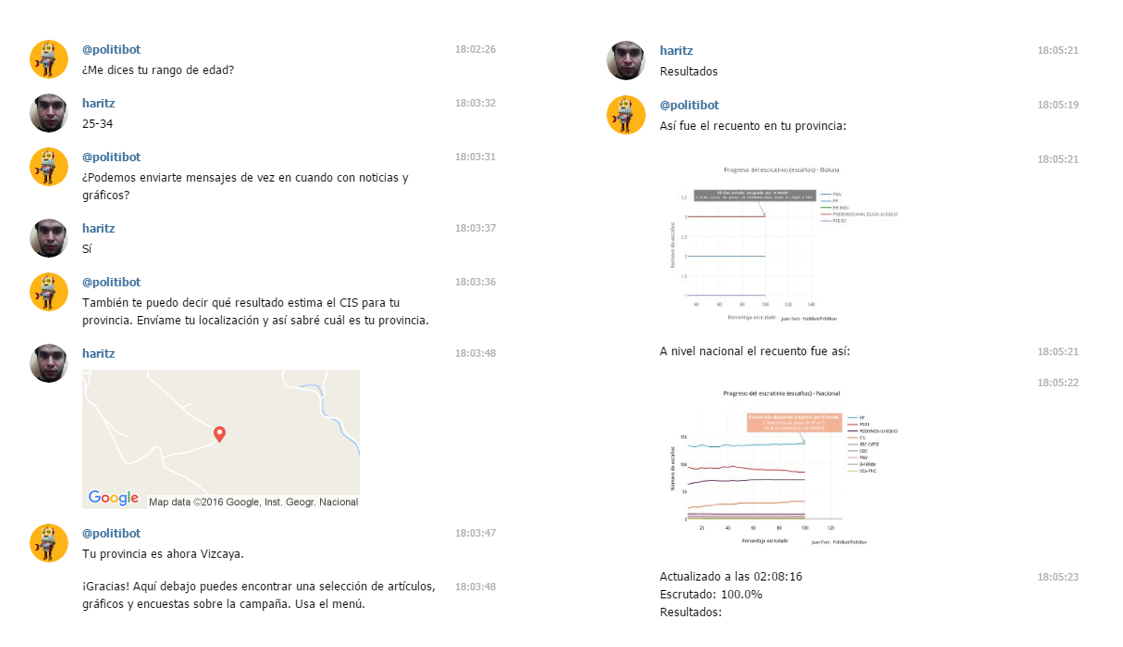
\includegraphics[width=0.8\textwidth]{./figs/Politibot.png}
	\caption{Un chatbot que informa sobre las elecciones españolas del 26-J ofreciendo información personalizada a cada usuario.}
	\label{fig:Politibot}
\end{figure}

Cualquiera puede pensar que los bots son un concepto nuevo dentro de las tecnologías de información. Sin embargo, es una idea que lleva desde los comienzos de la informática (uno de los pioneros fue el proyecto ELIZA\footnote{Proyecto ELIZA, un chatbot que simulaba a una psicóloga: \url{https://en.wikipedia.org/wiki/ELIZA}}), aunque en los últimos años está en crecimiento \cite{Ferrara2016}. Esto es debido al aumento de las redes sociales y de los dispositivos interconectados dentro de lo que se conoce cómo el Internet de las Cosas \footnote{Utilización de chatbots como interfaces para el Internet de las cosas: \url{https://iot.telefonica.com/blog/using-smart-chatbots-as-an-iot-interface}}.

Los chatbots proporcionan una interfaz de comunicación en la que se reduce el coste frente a la interacción humana \cite{Dans2016}. De igual manera también porque esta interacción ejerce menor presión en el usuario que quiere realizar consultas. Un bot está disponible para atender consultas 24 horas al día los 7 días de la semana, y puede atender simultáneamente consultas de múltiples usuarios, a diferencia de los humanos.

En el próximo Apartado \ref{sec:PlataformasChatbot} se hará hincapié en las plataformas que ofrecen los chatbots y las características de los mismos.

\section{Plataformas para desarrollo de agentes conversacionales}
\label{sec:PlataformasChatbot}

Como se ha mencionado en el apartado anterior, los chatbot existen desde hace varias décadas. Sin embargo, con el uso de las tecnologías móviles y el aumento del uso de aplicaciones de chat para conversar \cite{Montag2015}, ha hecho que los bots se hayan puesto en boga nuevamente.

Hay que diferenciar dos aspectos a la hora de hablar de plataformas para los chatbots. Por un lado existen las plataformas donde tiene el chatbot su interfaz, es decir, en qué aplicación o servicio mediante el cual chatea el usuario con el bot, que será en la que se centra este apartado. Por otro lado está la plataforma de desarrollo de los bots, que es la librería o servicio que se utiliza para desarrollar un chatbot que después será desplegado en una o más plataformas.

En referencia a la interfaz de los chatbots, en la actualidad muchas empresas ofrecen su plataforma como interfaz para interactuar con los chatbots. Entre ellas destacan: Facebook, Twitter, Telegram, Microsoft Skype o Slack. Sin embargo, empresas como Kik llevan trabajando años en el area de los chatbots \footnote{¿Como predijo Kik el crecimiento del uso de los chatbots? \url{https://backchannel.com/how-kik-predicted-the-rise-of-chat-bots-2eaf9027b86e}}.

La plataforma de desarrollo están muy ligada a la interfaz. Volviendo al ejemplo de politibot, en la Figura \ref{fig:PolitibotBotones} se observa como la interfaz de Telegram proporciona botones con las diferentes opciones que el usuario puede elegir para interactuar con el bot. Esta característica es particular de Telegram, que por ejemplo Slack no dispone. Sin embargo, otras plataformas ofrecen otras características que Telegram no contempla.
\begin{figure}[htb]
	\centering
	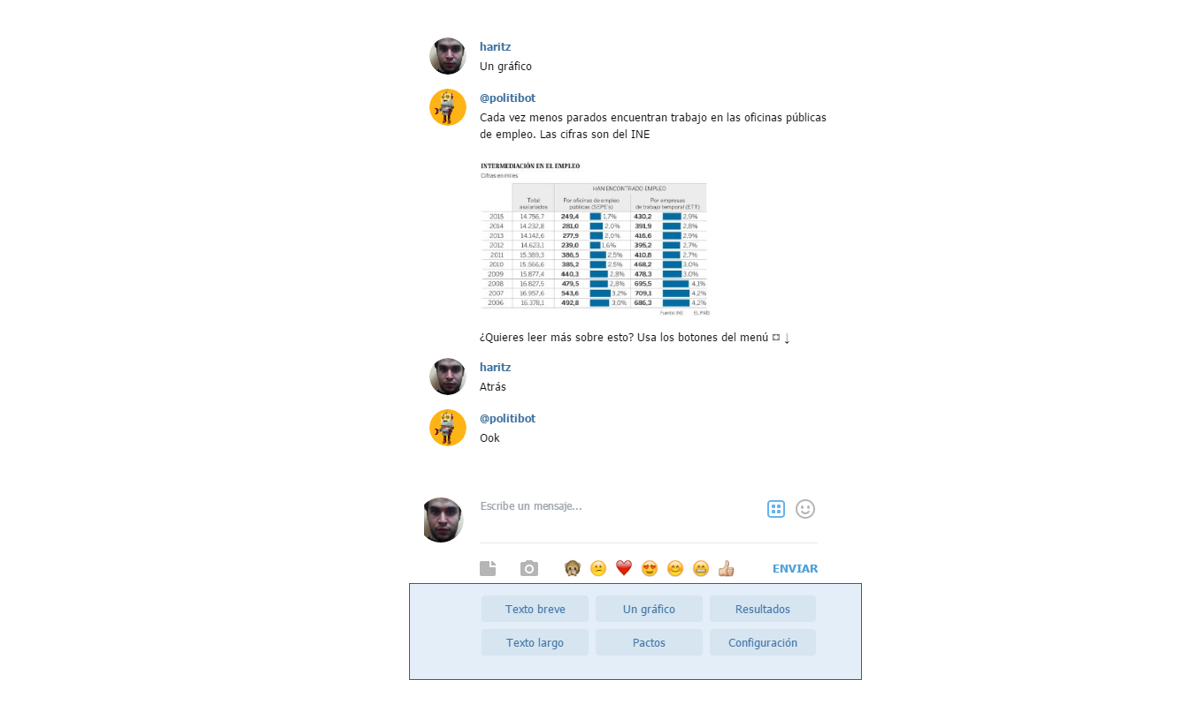
\includegraphics[width=0.8\textwidth]{./figs/PolitibotBotones.png}
	\caption{El chatbot define las posibles opciones que ofrece para responder mediante botones en lugar de esperar un mensaje textual.}
	\label{fig:PolitibotBotones}
\end{figure}

Es por ello que existen muchas plataformas de desarrollo. Algunas de ellas, como Microsoft Bot Framework \footnote{Microsoft Bot Framework: \url{https://dev.botframework.com/}} ofrecen soporte multiplataforma (Telegram, Slack, Skype, Messenger,...), otras como la API de Telegram\footnote{Telegram bot API: \url{https://core.telegram.org/bots}} es exclusiva para Telegram.

En este trabajo, se ha decidido trabajar con la librería Botkit \footnote{Sitio web de Botkit: \url{https://github.com/howdyai/botkit}}. Las principales razones son las siguientes:
\begin{itemize}
	\item Es multiplataforma, actualmente soporta Slack, Facebook Messenger\footnote{Sitio web de Facebook Messenger:\url{https://facebook.com/}} y Twilio IP Messaging\footnote{Sitio web de Twilio: \url{https://www.twilio.com/docs/api/ip-messaging}}.
	\item Es software libre, lo que permite ver el código fuente y modificarlo, además de que no tiene ningún coste económico.
	\item Es sencillo de desarrollar, permite abstraer bastante la implementación a bajo nivel de los chatbots, que es compleja debido a las llamadas asíncronas y las conexiones a múltiples servicios que trabaja por debajo.
\end{itemize}

Para profundizar en las características de implementación sobre Botkit es conveniente revisar el Capítulo \ref{cha:Implementation}.

\chapter{Análisis y diseño de la solución}
\label{cha:AnalysisAndDesign}

En este capítulo se hablará del análisis y del diseño adoptado para resolver el problema de generar chatbots. Para ello, como se ha mencionado previamente, se ha definido un artefacto llamado SheetChat. En el Apartado \ref{sec:Requisitos} se hablará de los requisitos que ha de tener el artefacto que permita generar bots. En el Apartado \ref{sec:FeatureModel} se realizará el análisis de las funcionalidades que ha de tener SheetChat. Finalmente, en el Apartado \ref{sec:DataModel} se mostrará cual es el modelo de datos a definir para la generación de agentes conversacionales basados en hojas de cálculo.

\section{Requisitos}
\label{sec:Requisitos}

\section{Modelo de características}
\label{sec:FeatureModel}

\section{Modelo de datos}
\label{sec:DataModel}

\subsection{Metamodelo}
\label{sec:Metamodel}

\subsection{Sintaxis concreta}
\label{sec:ConcreteSyntax}


\chapter{Implementación}

\section{Lenguaje de implementación}

\section{Botkit}

\section{Motor SQL para consultas. AlaSQL}

\chapter{Casos de estudio}
\label{cha:CaseStudies}

En este apartado se evaluará el funcionamiento del DSL definido para la creación de un SheetChat. Para ello se tienen que tener en cuenta todas las características previamente mencionadas, la definición del origen de datos, la creación de una conversación que nos proporcione una petición de datos de entrada y su salida asociada; y no menos importante, los recursos que nos permitan humanizar el bot para ofrecer una experiencia de usuario agradable.

Para ello se han elaborado tres ejemplos. El primero de ellos es dado las notas de dos asignaturas impartidas por un profesor, el poder preguntar por las notas de los alumnos. El segundo de los ejemplos permite dado un calendario de sesiones de un congreso científico, en este caso extraido del WISE de 2015\footnote{Calendario con las diferentes sesiones del congreso WISE: \url{http://www4.cis.fiu.edu/wise2015/@schema.html}}, poder obtener información sobre qué sesiones hay en los diferentes slots (u horarios). Por último, el tercer ejemplo permite, dada una hoja de cálculo autogenerada de una búsqueda de restaurantes de Miami en el sitio web Tripadvisor, obtener restaurantes por tipo de comida.

Los tres casos de estudio tendrán la misma estructura. En primer lugar se abordará el problema que el usuario tiene. En segundo lugar se realizará un análisis de las preguntas o cuestiones que tendrá que ser capaz de resolver el chatbot. Posteriormente se hará hincapié en la definición del DSL que tendrá que hacer el usuario. Finalmente se mostrará un ejemplo de interacción entre el chatbot generado y el usuario.

\section{Ejemplo 1: Notas de asignaturas impartidas por un profesor}
\label{sec:EjemploNotas}

Para el primer ejemplo la audiencia objetivo es un profesor de instituto que dispone de las notas de sus alumnos almacenadas en hojas de cálculo. Él es profesor de dos asignaturas Matemática y Física.

\subsection{Hoja de cálculo con los datos}

Para el almacenamiento de las notas de sus alumnos dispone de dos hojas de cálculo, una con las notas de Matemática (ver Figura \ref{fig:SheetNotasMate}) y otra para las calificaciones de la asignatura de Física (ver Figura \ref{fig:SheetNotasFisica}).

Tal y como se puede observar en la Figura \ref{fig:SheetNotasMate} el profesor tiene las notas de cada uno de sus alumnos que va rellenando a medida que se les evalúa de los diferentes aspectos de las asignaturas. Por lo tanto, cada fila representa a un alumno y cada columna a cada concepto a evaluar de la asignatura.

En el método de evaluación empleado por el profesorado se tiene en cuenta trabajos de clase o ejercicios y exámenes durante la evaluación continua. En caso de que la media ponderada de estos parciales supere un 5 el alumno habrá aprobado mediante la evaluación continua. En caso contrario, tendrá que presentarse a un examen final con todo el temario del curso. A modo de ejemplo se puede visualizar en la Figura \ref{fig:SheetNotasMate} como el alumno Adrian Arana ha aprobado la evaluación continua con un 5.9 mientras que Alberto Ballester tuvo que presentarse al examen final para aprobar dado que en la evaluación continua su nota era de 3.85.

\begin{figure}[htb]
	\centering
	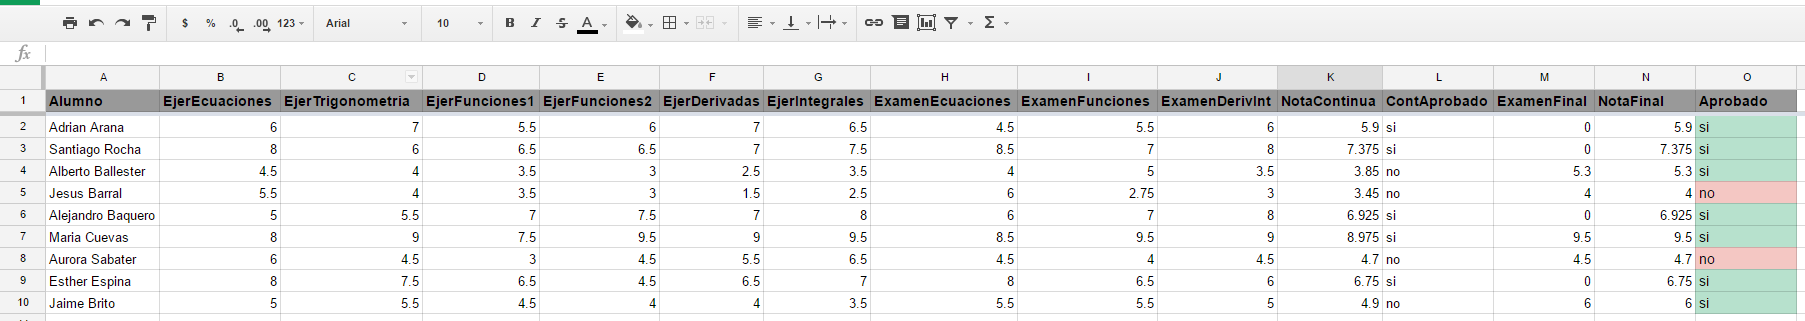
\includegraphics[width=0.8\textwidth]{./figs/sheetNotasMate.png}
	\caption{Hoja de cálculo del profesor para la asignatura de matemática.} \label{fig:SheetNotasMate}
\end{figure}

\begin{figure}[htb]
	\centering
	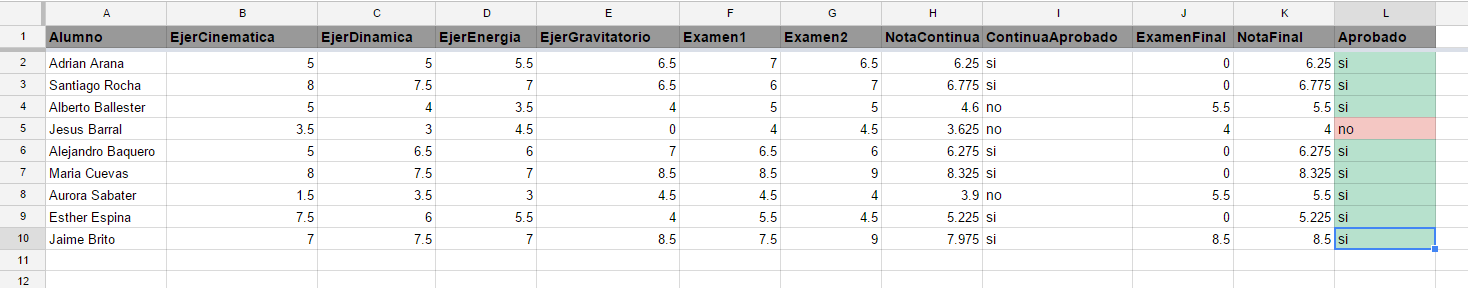
\includegraphics[width=0.8\textwidth]{./figs/sheetNotasFisica.png}
	\caption{Hoja de cálculo del profesor para la asignatura de física.} \label{fig:SheetNotasFisica}
\end{figure}

\subsection{Análisis de preguntas}
\label{sec:queriesNotas}

Una vez conocidos los datos almacenados, el profesor que quiere generar un chatbot tiene que tener en cuenta qué tipo de análisis quiere hacer sobre los datos, o dicho de otra manera, qué consultas va a realizar sobre los datos. Debería de ser capaz de decidir cuales son las preguntas más habituales sobre esos datos o las que más frecuentemente le piden sus alumnos. Dado que son asignaturas diferentes y su método de evaluación no es exactamente el mismo, las preguntas que se puede llegar a realizar también son diferentes.

A continuación se recogen algunas de las preguntas que podría hacer el profesor:
\begin{itemize}
	\item \textbf{¿Cuál es la nota que tiene un alumno en cada uno de los ejercicios de mate/fisica?} Es habitual preguntar por la nota en uno de los ejercicios o en el conjunto de los mismos a lo largo de la evaluación.
	\item \textbf{¿Cuál es la nota de un alumno en los exámenes parciales de mate/física?} Al igual que sucede con los ejercicios, es interesante conocer las notas de los exámenes parciales.
	\item \textbf{¿Se debe de presentar un alumno al examen final de mate?} O dicho de otra manera, ¿ha aprobado la evaluación continua?
	\item \textbf{¿Qué nota debe de sacar un alumno en los exámenes de física para aprobar la asignatura?} O preguntado de otra manera, ¿Qué nota ponderada tiene en los ejercicios de evaluación continua?
	\item \textbf{¿Ha aprobado un alumno la asignatura de física?} De esta manera se sabe si un alumno ha de presentarse a la segunda convocatoria de física o no.
\end{itemize}

\subsection{Definición del DSL}

Como se ha comentado en el Capítulo \ref{cha:AnalysisAndDesign} hay que definir mediante el uso del DSL de SheetChat el origen de los datos y los intents para cada una de las consultas que se quiera extraer de la hoja de cálculo previamente definidas en el Apartado \ref{sec:queriesNotas}.

Si se observa la Figura \ref{fig:DSLNotas} se puede observar cómo es la definición de las hojas de cálculo a consultar. De igual manera se define una descripción para el chatbot y un mensaje de bienvenida que nos ayude a recordar alguna de las funcionalidades del bot. Posteriormente se muestra un intent de los que deberá de definir el profesor que vaya a utilizar el chatbot.

El intent a resolver es el de obtener la nota de los ejercicios de mate de un determinado alumno. El origen de datos por tanto será la hoja de NotasMate. Se define que las columnas que el bot debe de responder son las de los ejercicios. También se define que sólo se desea un resultado, ya que sólo se pregunta por un alumno concreto. Esta característica es útil para mostrar un número determinado de resultados. En este caso cada alumno se identifica inequívocamente por el nombre y apellido. También se indica que se muestre el nombre de la columna (en este caso el nombre del ejercicio).

Dentro del intent también se definen las entidades de filtrado. En este caso se define la columna Alumno. El tipo de filtrado utilizado es LIKE, que tiene la misma funcionalidad que el like de SQL. Esto permite no tener que introducir nombre y apellido del alumno, si no introducir parcialmente su nombre a la hora de filtrar. En lugar de exigir al usuario escribir Adrian Arana, podrá preguntar por las notas de Adrian o de Arana. Por último se definen mensajes que permitan al usuario preguntar de una manera más amigable (o humana, ver Apartado \ref{sec:Humanization}) por las entidades que hacen falta.

\begin{figure}[htb]
	\centering
	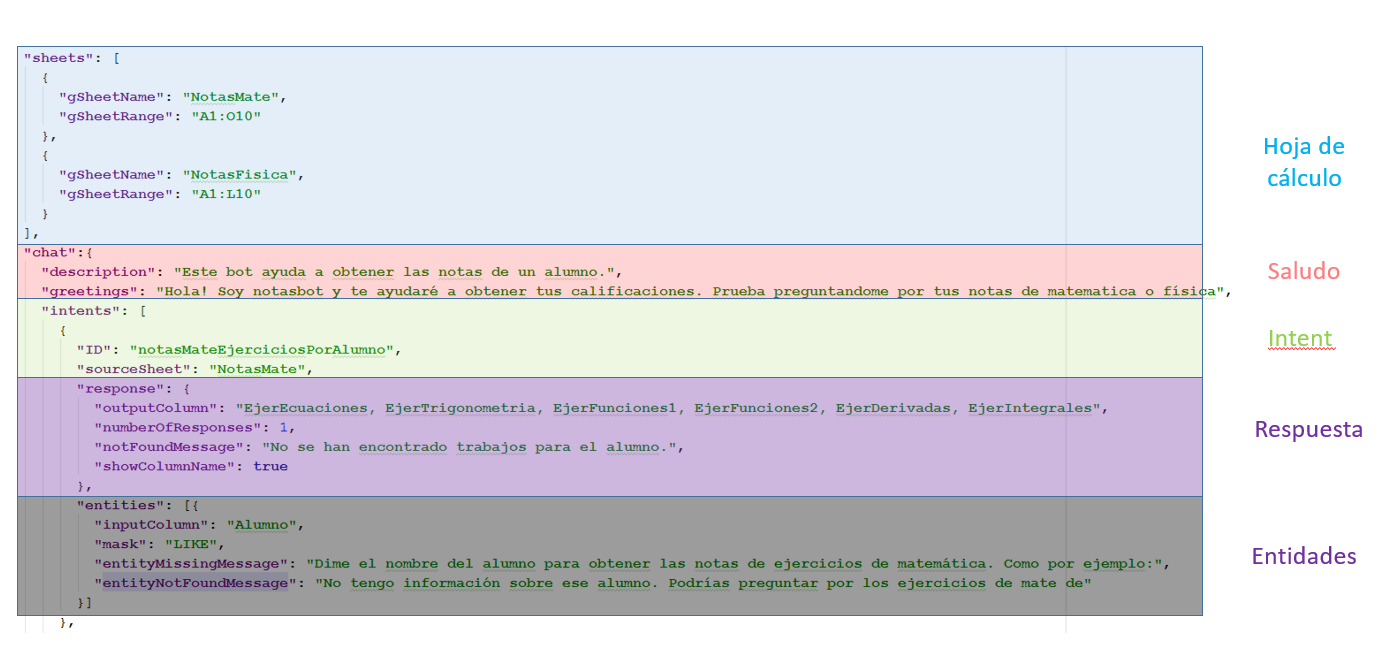
\includegraphics[width=1.2\textwidth]{./figs/DSLNotas.png}
	\caption{DSL con la definición de las Sheet y un intent a utilizar en el ejemplo de notas.}
	\label{fig:DSLNotas}
\end{figure}

Algunas preguntas son más difíciles de formular debido a la naturaleza de los datos. Sin embargo, SheetChat ofrece algunos mecanismos que permiten resolver funciones matemáticas a la hora de realizar consultas sobre los datos. Se puede observar en la pregunta relacionada con obtener la nota ponderada. La nota ponderada de los ejercicios de Física el profesor lo tiene definido de una manera determinada. Esto no es una columna como tal dentro de la hoja de cálculo, si no que es una entidad derivada. En la Figura \ref{fig:DSLNotasPonderada} se observa que dentro del response hay una expresión matemática que define qué es la nota ponderada de los ejercicios. De igual manera, en las respuestas se puede proporcionar un mensaje personalizado para mejorar la humanización del bot ofreciendo una respuesta más sencilla de interpretar por un humano.

\begin{figure}[htb]
	\centering
	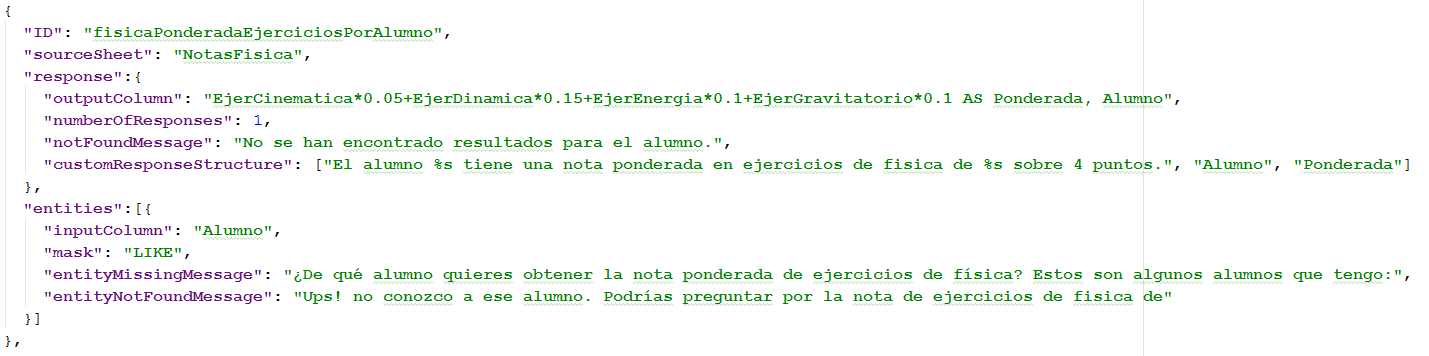
\includegraphics[width=0.8\textwidth]{./figs/DSLNotasPonderada.png}
	\caption{Definición de la pregunta para obtener la nota ponderada de los ejercicios de física del ejemplo de notas.}
	\label{fig:DSLNotasPonderada}
\end{figure}

\subsection{Ejemplo de uso del chatbot}

A continuación se puede visualizar cómo sería un ejemplo de interacción entre un ser humano y el bot que se ha generado a partir del DSL de SheetChat en el ejemplo de las notas. En la Figura \ref{fig:EjecucionNotas1} se puede observar un intercambio de mensajes para obtener información respecto al alumno Alberto. En primer lugar se ha saludado al chatbot para que este proporcione su mensaje de bienvenida. Esta interacción no es necesaria si se conocen cuales son las características del chatbot. Posteriormente se le han preguntado por los resultados de alberto en matemática: si habia aprobado la evaluación continua y las notas que ha obtenido para conocer la causa de su suspenso. De igual manera se han realizado dos preguntas respecto a las notas de física.

\begin{figure}[htb]
	\centering
	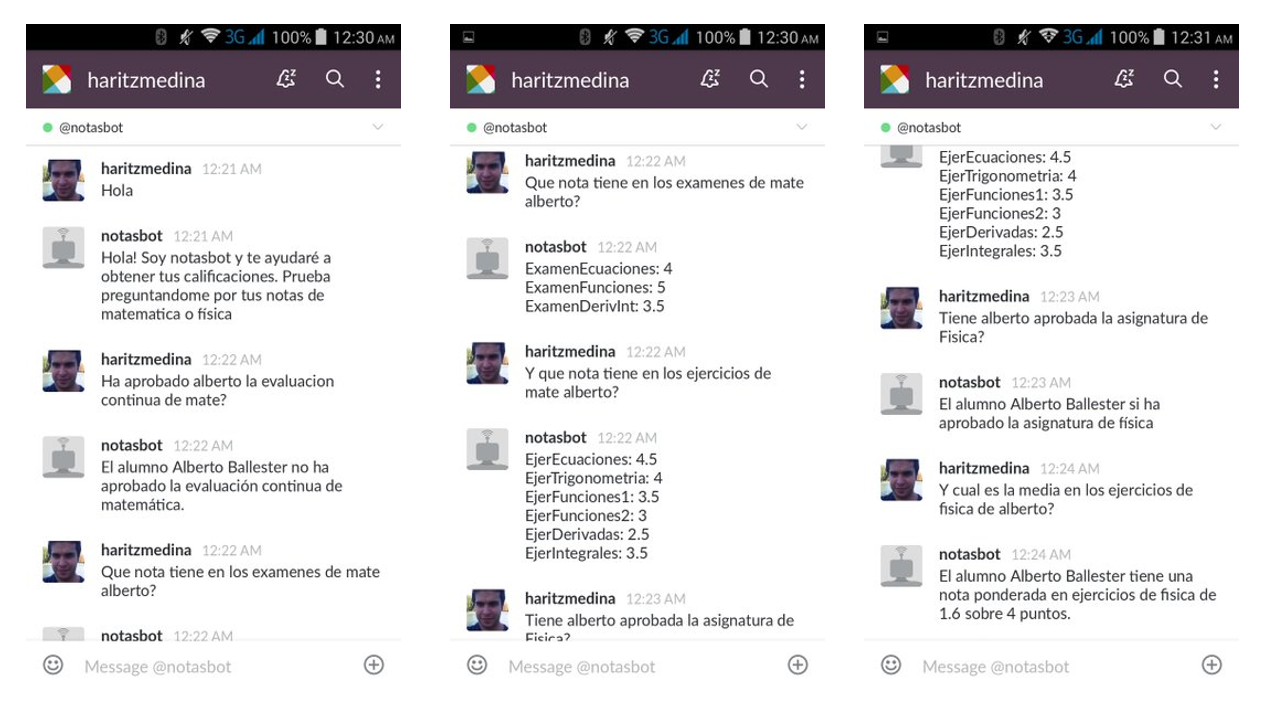
\includegraphics[width=0.8\textwidth]{./figs/ejecucionNotas1.png}
	\caption{Interacciones del usuario a la hora de consultar las notas de Alberto.}
	\label{fig:EjecucionNotas1}
\end{figure}

En este caso el chatbot ha inferido cuales eran los intents del usuario y a su vez la entidad necesaria para cada una de ellas, en este caso el nombre del alumno. Si se obtienen de la frase de manera adecuada los intents y las entidades el chatbot proporciona la respuesta. En caso de que se haya inferido el intent pero no las entidades, preguntará por ellas (ofreciendo sugerencias que ayuden al usuario). Esto sucede en la Figura \ref{fig:EjecucionNotas2} dado que no se le había proporcionado ningún nombre a la hora de preguntar por la media en los ejercicios de física. De igual manera, si se le proporciona un nombre no existente, el chatbot le seguirá ofreciendo sugerencias.

\begin{figure}[htb]
	\centering
	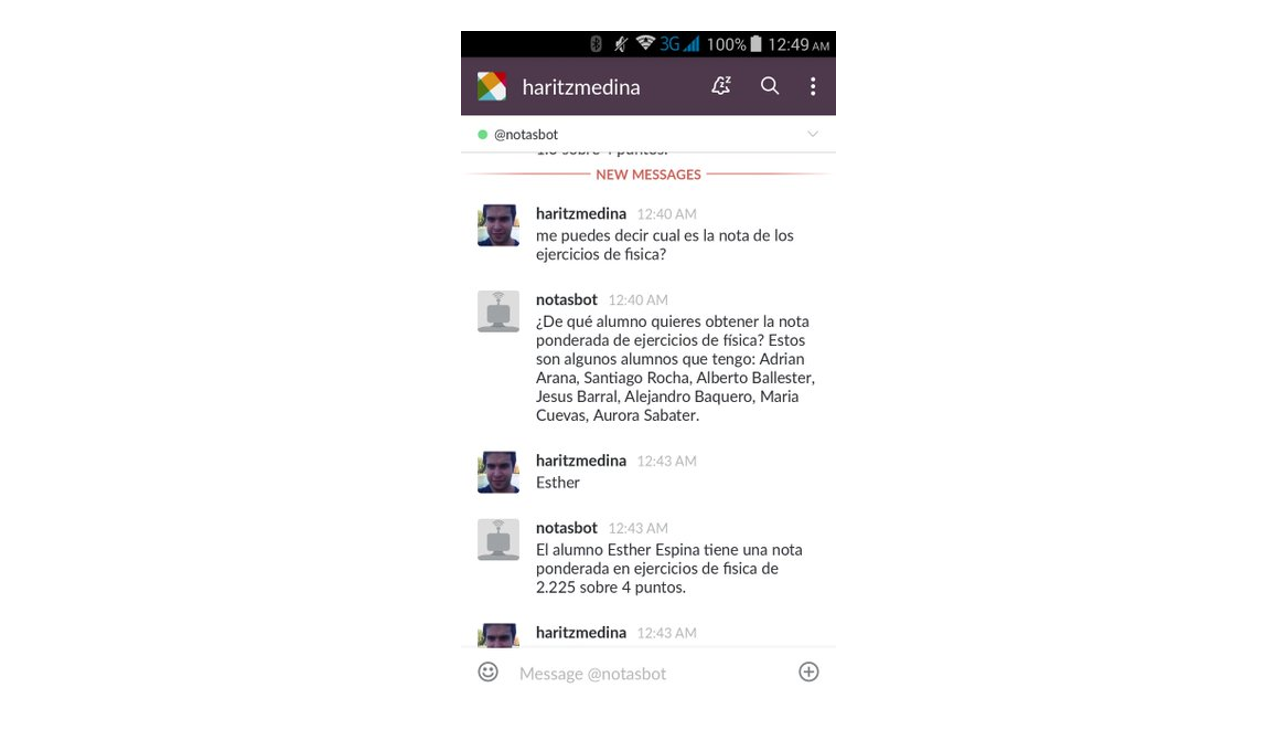
\includegraphics[width=0.8\textwidth]{./figs/ejecucionNotas2.png}
	\caption{El chatbot recomienda algunos nombres en caso de que no se defina o se defina un nombre inexistente para hacer el filtrado en la hoja de cálculo.}
	\label{fig:EjecucionNotas2}
\end{figure}

\section{Ejemplo 2: Calendario de sesiones en un congreso científico}

Los congresos disponen de un calendario complejo, dónde hay trabajos más o menos interesantes o relevantes con la rama de especialización que tiene el asistente. Es por ello que acudir a las sesiones más afines a tu trabajo es importante. Es interesante disponer de información in situ de cuales son las próximas charlas que habrá, dónde o quién las presenta. Sin embargo, los sitios webs rara vez están preparados para su navegación por el móvil o se pierde mucho tiempo en encontrar los eventos a los que se desea acudir. Es una información relevante y que se desea conocer en el momento.

Este ejemplo se centra en ofrecer una alternativa en forma de bot mediante una hoja de cálculo creada a partir del horario de la conferencia WISE 2015 \footnote{Programa del WISE 2015 (Web Information System Engineering) \url{http://www4.cis.fiu.edu/wise2015/@schema.html}}.

\subsection{Hoja de cálculo con los datos}

Como se ha mencionado previamente la hoja de cálculo es creada a partir de una tabla con el programa disponible en el sitio web. En la Figura \ref{fig:SheetConference} se puede observar el calendario de las diferentes sesiones que están presentes en el congreso. Cada sesión tiene asociada un día y un slot (una franja horaria) donde se exponen trabajos. En algunos de los slots se produce un solapamiento de múltiples sesiones, por lo que es interesante que el usuario conozca cuales son las charlas para elegir la más interesante.

\begin{figure}[htb]
	\centering
	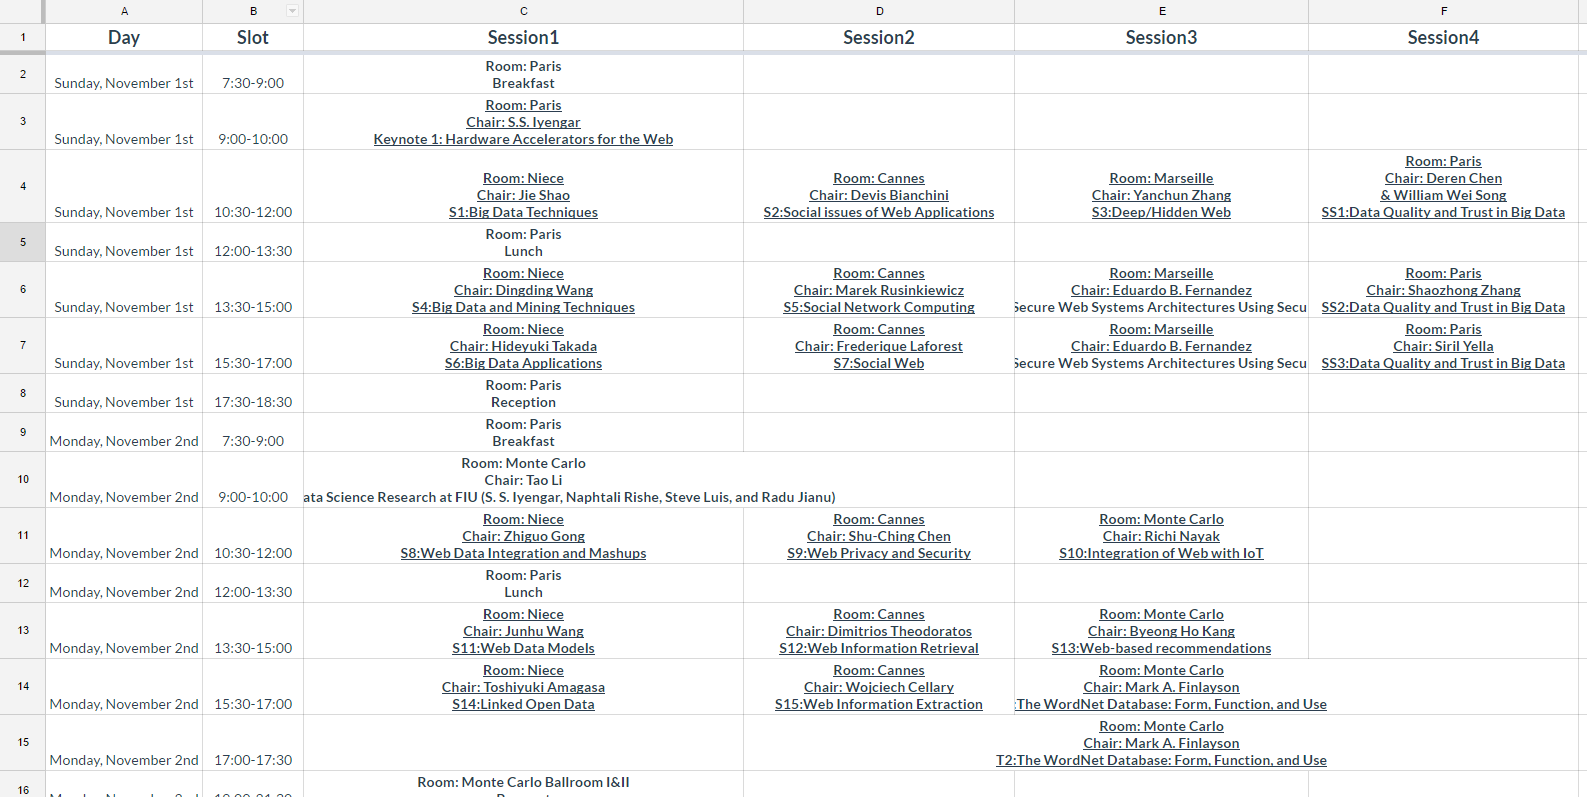
\includegraphics[width=0.8\textwidth]{./figs/sheetConference.png}
	\caption{Hoja de cálculo con el programa del WISE 2015.}
	\label{fig:SheetConference}
\end{figure}

\subsection{Análisis de preguntas}

Como se ha comentado previamente, el usuario del bot tiene como objetivo poder conocer el programa del congreso durante la estancia en él. Algunas de las preguntas que le pueden surgir durante el evento están recogidas a continuación:
\begin{itemize}
	\item \textbf{¿Cuáles son las charlas en un horario concreto, es decir, qué eventos hay en esa franja horaria?} De los eventos que existan en esa franja horaria, el asistente al congreso podría decantarse por la que más interesante le resulte.
	\item \textbf{¿Qué eventos hay relacionados con un tema (o topic) en particular?} De esta manera el usuario sabrá con una simple pregunta en qué horarios están programadas charlas interesantes para él.
	\item \textbf{¿Quiero conocer en qué sesiones participa una persona?} Los investigadores conocen el trabajo de algunas personas y puede interesarle saber si estas personas participan como expertas en la materia de una determinada sesión.
\end{itemize}

\subsection{Definicion del DSL}

El diseño del chatbot en este ejemplo constará de una única hoja de cálculo y de dos intents. A pesar de que previamente se han definido 3 cuestiones, sólo hace falta definir dos intents debido a que la obtención de las sesiones relacionadas con un tema en concreto o presidido por un chairman concreto se pueden unir en una. Esto es debido a la naturaleza de los datos. Una columna sesión tiene como valor un string que incluye ambas informaciones. A la hora de realizar el filtrado, se filtra por valor de la columna que se desee. Visto en un ejemplo, observando la sesión 1 del domingo en el slot 10:30-12:00, es lo mismo filtrar por el topic \emph{Hardware Accelerators for the Web} por la habitación \emph{Paris} o el chairman \emph{Iyengar}, se obtendrá como resultado el dia y slot de esa sesión.

Por otro lado, en este ejemplo, surge la novedad de filtrar por más de una columna. En la Figura \ref{fig:DSLConference} se observa remarcado en color azul el entity definido. En este caso se han definido cuatro columnas que actuarán como filtro. A la hora de preguntar por el topic o chairman, el chatbot buscará si se dan positivos en cualquiera de las cuatro columnas. En caso de que el valor introducido por el usuario dé positivo por alguna de las cuatro columnas, se le mostrará el día y la hora (o slot) de ese evento.

\begin{figure}[htb]
	\centering
	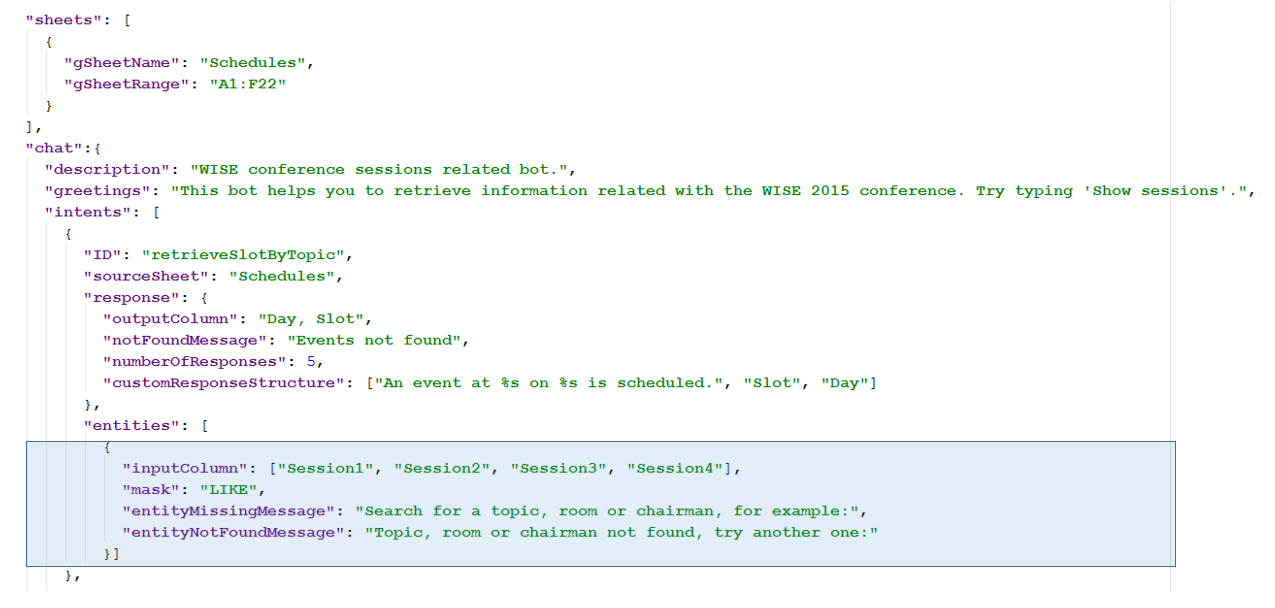
\includegraphics[width=0.8\textwidth]{./figs/DSLConference.png}
	\caption{Implementación del chatbot de la conferencia. Cabe destacar remarcado en azul el intent con input multicolumna.}
	\label{fig:DSLConference}
\end{figure}

\subsection{Ejemplo de uso del chatbot}

A continuación se presenta un ejemplo de interacción real con el chatbot desarrollado para el programa de las conferencias. Para la obtención de las sesiones en una franja horaria concreta, tal y como se ha mencionado en la implementación del chatbot, se requiere de dos parámetros (el día y el slot). En la Figura \ref{fig:EjecucionConference} el Chatbot guía al usuario mediante preguntas para obtener la información suficiente de a qué slot se refiere el usuario. En este caso realiza una pregunta respecto a los días y otra respecto al slot. Si el usuario hubiese añadido esa información a la hora de hacer la pregunta, el chatbot podría haber inferido estas entidades y ahorrarse los pasos de preguntarlo. Esto es lo que sucede en la pregunta de la imagen derecha, donde el usuario ha proporcionado un criterio de búsqueda.

\begin{figure}[htb]
	\centering
	\includegraphics[width=0.8\textwidth]{./figs/EjecucionConferencia.png}
	\caption{Interacción del usuario a la hora de preguntar por los eventos en una hora concreta (Imagen izquierda y central) y consulta respecto a un topic concreto (Imagen derecha).}
	\label{fig:EjecucionConference}
\end{figure}


\section{Ejemplo 3: Búsqueda de restaurantes de Tripadvisor}

En este tercer caso de estudio se muestra además de un nuevo contexto de uso, el uso de un origen de datos web. En la actualidad la mayoría de información se puede recabar en la red, sin embargo esta no suele tener una estructura utilizada en un ámbito general como son las tablas de bases de datos o las hojas de cálculo.

En este ejemplo se mostrará cómo se pueden realizar búsquedas en restaurantes extraídos del sitio web Tripadvisor. Tripadvisor es un sitio web de opinión sobre hoteles, restaurantes, y otros lugares de ocio. En su web se pueden filtrar los resultados en base a localización (como una ciudad o provincia), características del sitio (número de estrellas de un hotel o tipo de comida de un restaurante) y otros muchos aspectos. Concretamente en este ejemplo se ha realizado una búsqueda de restaurantes en Miami (Estados Unidos), que es lo que se puede observar en la Figura \ref{fig:TripadvisorMiami}.

\begin{figure}[htb]
	\centering
	\includegraphics[width=0.8\textwidth]{./figs/tripadvisorMiami.png}
	\caption{Búsqueda de restaurantes de Miami en Tripadvisor}
	\label{fig:TripadvisorMiami}
\end{figure}

La idea para este ejemplo es demostrar que estos datos en la web pueden ser extraidos a una hoja de cálculo y generar un chatbot mediante la herramienta SheetChat.

\subsection{Hoja de cálculo con los datos}

Como se ha mencionado al comiendo de este caso de estudio, el objetivo es poder representar estos datos en forma de hoja de cálculo. Para ello en la web existen múltiples herramientas de web scraping (extracción de información de la web). A pesar de que la web de tripadvisor muestre los restaurantes en un formato más amigable para el ser humano, si que todos los restaurantes comparten una estructura similar. En la Figura \ref{fig:TripadvisorMiami} se observa que todos los restaurantes tienen un hyperlink con el nombre del restaurante donde pinchando saldría la ficha del restaurante en cuestión. Cada restaurante tiene una imagen asociada, un número de opiniones, dos breves opiniones, el precio promedio del menú del restaurante y el tipo de comida. Precisamente, el encontrar patrones y extraer datos es el objetivo de herramientas como Import.io\footnote{\href{https://www.import.io/}{Import.io} extracción de datos tabulares a partir de sitios web.}.

El funcionamiento de import.io permite extraer una tabla con los resultados de la búsqueda de restaurantes de Miami. En el Anexo \ref{anx:importio} se puede profundizar en el funcionamiento de la herramienta. Para el ejemplo, simplemente la hoja de cálculo que obtenemos es la presentada en la Figura \ref{fig:SheetTripadvisor}. Mediante import.io se han extraido 400 restaurantes en Miami. En la tabla se pueden observar las columnas sobre las que podremos realizar preguntas posteriormente al bot, nombre del restaurante (Name), sitio web con la ficha de Tripadvisor (url), rango de precios de los menús (RangePrice) o tipo de comida (Cuisines).

\begin{figure}[htb]
	\centering
	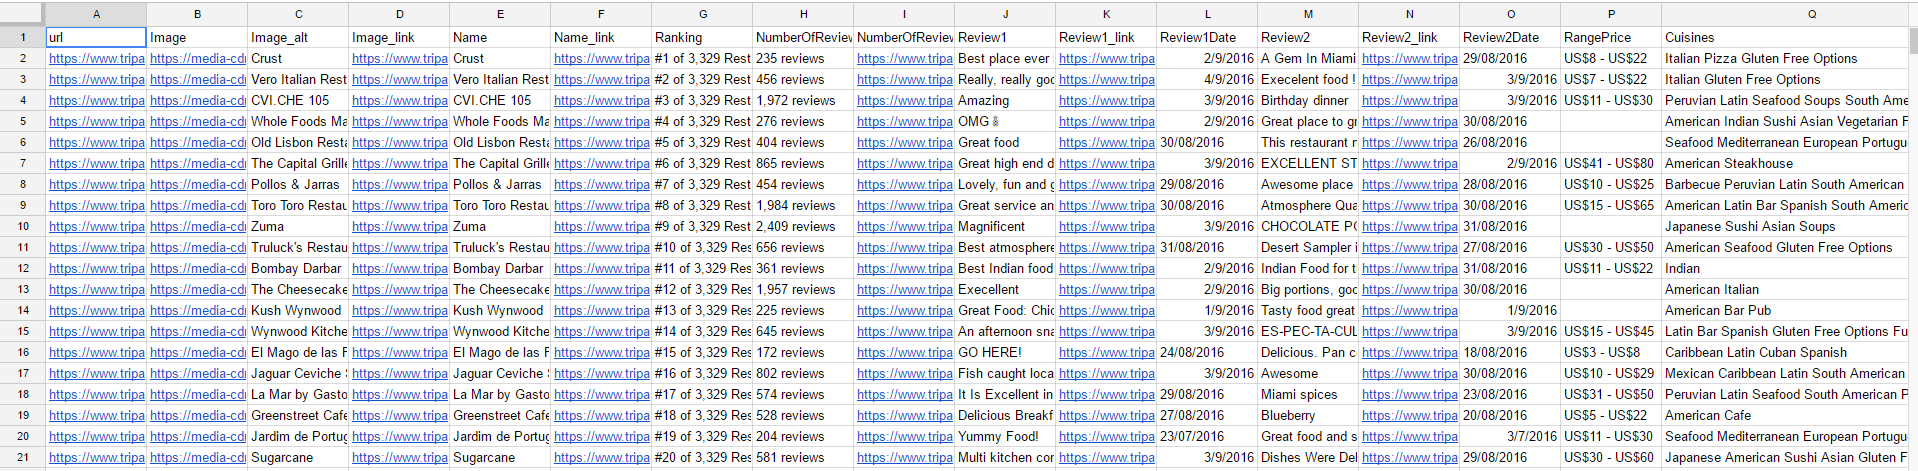
\includegraphics[width=0.8\textwidth]{./figs/sheetTripadvisor.png}
	\caption{Hoja de cálculo con restaurantes de Miami extraidos de Tripadvisor.}
	\label{fig:SheetTripadvisor}
\end{figure}

\subsection{Análisis de preguntas}

Tras observar los datos extraídos de Tripadvisor, el usuario podría hacer diferentes preguntas. En este caso se ha decidido que pueden ser interesantes las que se presentan a continuación:
\begin{itemize}
	\item \textbf{¿Me podrías ayudar a buscar restaurantes con comida italiana?} Al igual que se puede preguntar por italiana, se puede preguntar por cualquier tipo de comida que se haya extraído de los restaurantes situados en Miami.
	\item \textbf{¿Qué restaurantes vegetarianos hay por menos de 45 dolares?} Similar a la pregunta anterior, con la condición de precio máximo, ya que son dos aspectos que se suelen mirar frecuentemente a la hora de buscar un restaurante, si gusta la comida y el precio.
	\item \textbf{¿Qué opinión hay sobre un restaurante concreto?} Mediante la opinión de otros usuarios extraída del sitio web, el usuario del Chatbot puede deducir si un restaurante es bueno o no.
\end{itemize}

\subsection{Definicion del DSL}
\label{sec:DSLTripadvisor}

Para este ejemplo se trabajará la definición de las interacciones para las dos primeras cuestiones previamente definidas. En la Figura \ref{fig:DSLTripadvisor1} se ve la definición para la primera de las preguntas, dónde la entidad de entrada es la columna \emph{Cuisines} (tipo de cocina) y en la salida se mostrará un mensaje personalizado con el nombre, el tipo de comida, el rango de precio y un link para abrir la ficha en Tripadvisor.

Se ha observado que el resultado que ofrece el chatbot (junto con la previsualización de links de la plataforma Slack) hace que el chatbot al ofrecer la respuesta sea muy verboso. Por esa razón, se ha decidido que se limite a tres el número de respuestas máximas que va a recibir el usuario.

\begin{figure}[htb]
	\centering
	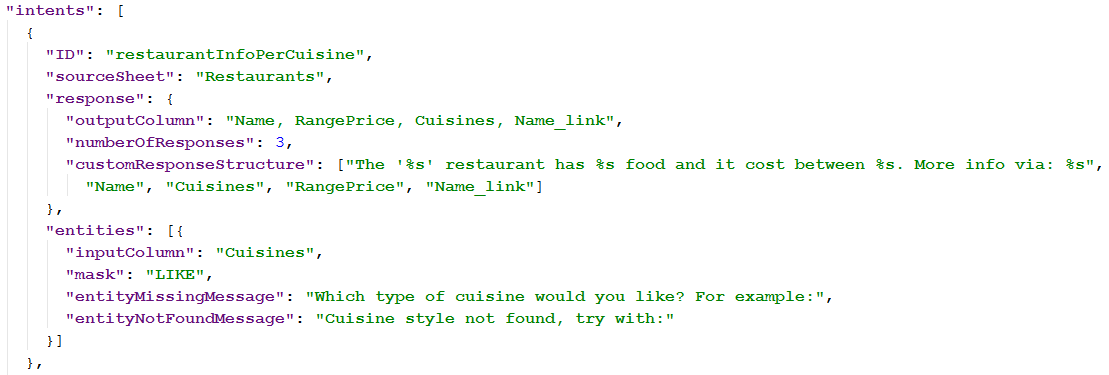
\includegraphics[width=0.8\textwidth]{./figs/DSLTripadvisor1.png}
	\caption{DSL de SheetChat que describe el intent para la búsqueda por tipo de comida de los restaurantes de Tripadvisor.}
	\label{fig:DSLTripadvisor1}
\end{figure}


De igual manera, en la Figura \ref{fig:DSLTripadvisor2} se muestra la definición utilizando el DSL de SheetChat donde el usuario hará peticiones respecto a un precio máximo y un tipo de comida concretos, es decir, hay dos entidades participantes a la hora de realizar el filtrado entre los 400 restaurantes. Como novedad cabe destacar que el valor del campo Mask en lugar de ser LIKE (que sirve para comparar strings), se utiliza el símbolo < para designar que es un valor númerico y que el filtro rechazará los resultados mayores que el precio máximo delimitado por el usuario a la hora de interaccionar con el Chatbot, tal y cómo se muestra en el Apartado \ref{sec:EjemploUsoTripadvisor}.

\begin{figure}[htb]
	\centering
	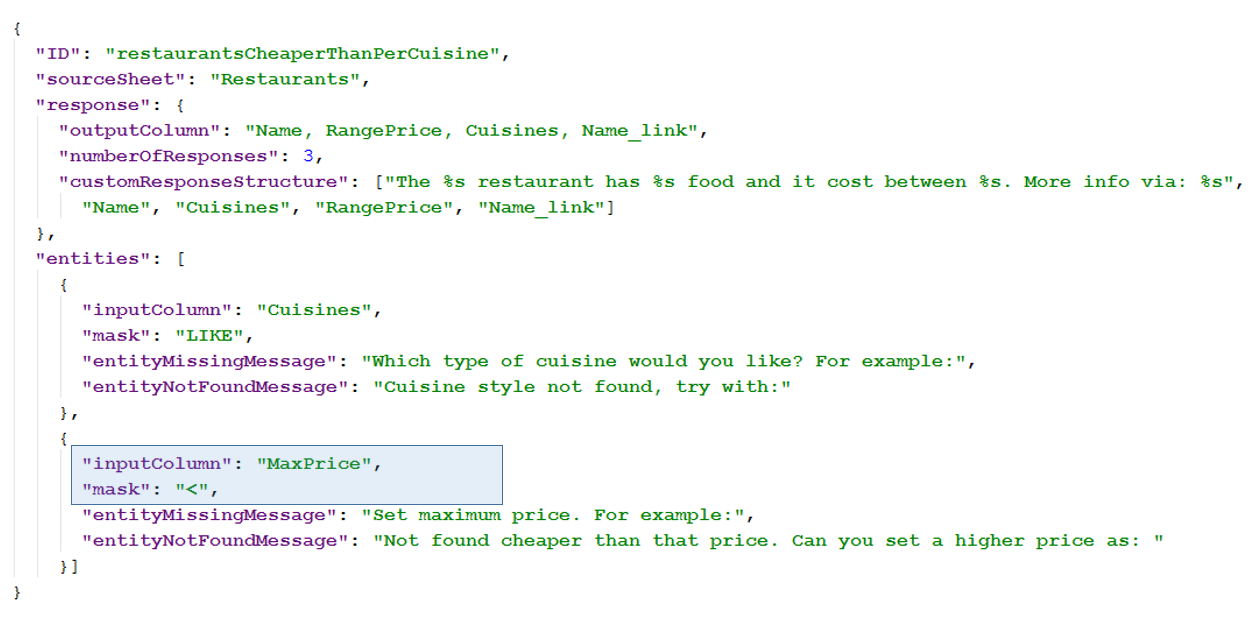
\includegraphics[width=0.8\textwidth]{./figs/DSLTripadvisor2.png}
	\caption{DSL de SheetChat que describe el intent para la búsqueda por precio máximo (resaltado en azul) y tipo de comida de los restaurantes de Tripadvisor.}
	\label{fig:DSLTripadvisor2}
\end{figure}

\subsection{Ejemplo de uso del chatbot}
\label{sec:EjemploUsoTripadvisor}

Tras el diseño del Chatbot mediante el DSL de SheetChat a continuación se presenta cómo sería la experiencia de uso de este chatbot por parte de un usuario.

En la Figura \ref{fig:EjecucionTripadvisor1} el usuario en primer lugar saluda al Chatbot y este le ofrece alguna de sus funcionalidades por si acaso el usuario no se acuerda de qué trata este chatbot o qué funcionalidades tenía. Posteriormente se dispone a preguntar por restaurantes italianos. El chatbot le responde con tres resultados, el número máximo de resultados que se indicó en el diseño del chatbot (ver Apartado \ref{sec:DSLTripadvisor}).

\begin{figure}[htb]
	\centering
	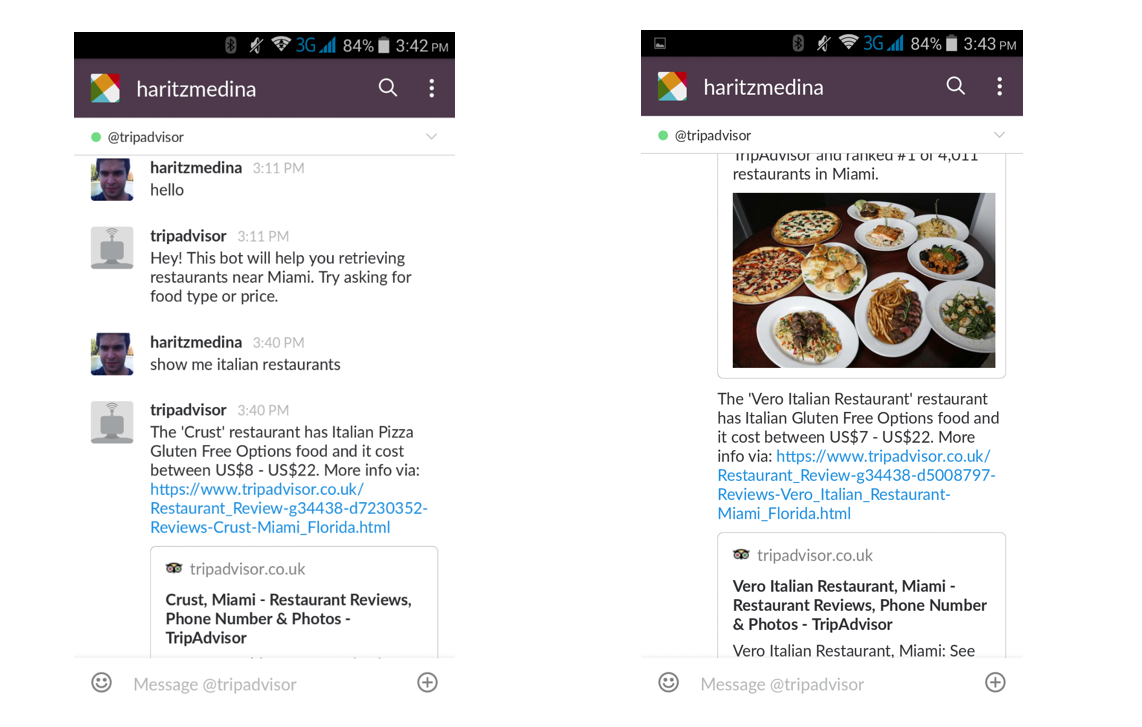
\includegraphics[width=0.8\textwidth]{./figs/ejecucionTripadvisor1.png}
	\caption{Interacción entre el usuario y el chatbot que recomienda restaurantes en base a un tipo de cocina.}
	\label{fig:EjecucionTripadvisor1}
\end{figure}

En la interacción de la Figura \ref{fig:EjecucionTripadvisor2} se observa que al usuario las recomendaciones de los restaurantes italianos le ha resultado cara. Por lo tanto decide preguntar por restaurantes con precio menor a 15 dolares. El chatbot ha detectado que el usuario está preguntando por restaurantes con un precio máximo y un tipo de cocina determinado. El chatbot restringe las respuestas en base a ese nuevo filtro y muestra el único restaurante que cumple esas características. En caso de que no hubiese ningún restaurante que cumpliese ambos criterios preguntaría por las entidades nuevamente.

\begin{figure}[htb]
	\centering
	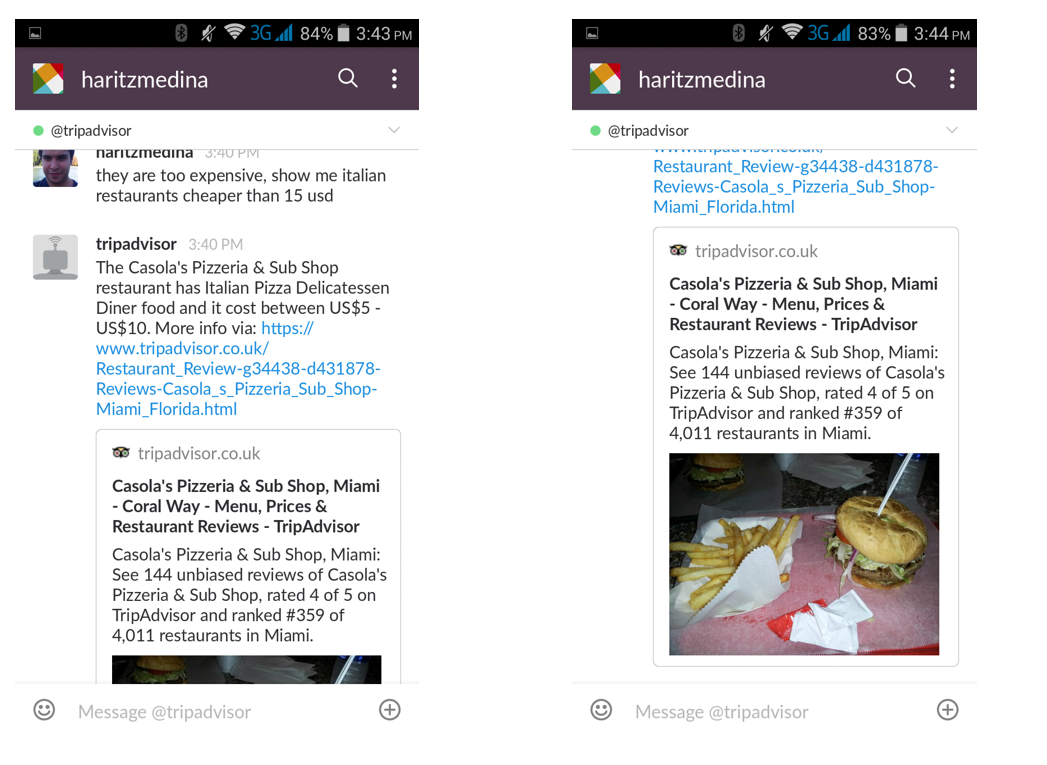
\includegraphics[width=0.8\textwidth]{./figs/ejecucionTripadvisor2.png}
	\caption{El bot de Tripadvisor recomienda restaurantes italianos con precio menor a 15 dolares por petición del usuario.}
	\label{fig:EjecucionTripadvisor2}
\end{figure}

De esta manera, mediante el uso de un chatbot, el usuario evita tener que aplicar filtros en el sitio web de Tripadvisor que en una configuración móvil suele resultar en lineas generales bastante farragoso.

\chapter{Trabajo Futuro y Conclusiones}
\label{cha:FutureWorkAndConclusions}

En este capítulo se divide en dos apartados. En el Apartado \ref{sec:FutureWork} se hablará del trabajo futuro y de las mejoras que se puedan aplicar a este trabajo. En el Apartado \ref{sec:Conclusions} se extraerán unas conclusiones obtenidas durante el desarrollo del trabajo.

\section{Trabajo futuro}
\label{sec:FutureWork}

El trabajo presentado en este proyecto sirve como prueba conceptual para demostrar que la solución al problema detectado puede ser factible. Está claro que un componente que demostrará, si además de ser factible, es útil es la evaluación de la propia herramienta con usuarios de hoja de cálculo. Es por ello que resulta difícil de vaticinar cuales son los siguientes pasos a dar en el desarrollo de esta idea, ya que irán claramente asociada a esa evaluación y feedback que puedan proporcionar los usuarios.

Sin embargo, a lo largo del desarrollo se han detectado algunos aspectos de mejora en lo que a la herramienta se refiere. En concreto se han dividido en los siguientes aspectos: enriquecimiento del diseño del DSL, usabilidad de los chatbot generados, el ecosistema de plataformas utilizado para su desarrollo y la actualización de los datos de las hojas de cálculo.

\subsection{Diseño del DSL}

El DSL diseñado permite la creación de consultas abstrayendo al usuario del conocimiento de un lenguaje como es SQL. A pesar de que esto resulta positivo, se ha detectado que el actual diseño del DSL no permite realizar consultas que puede que sean bastantes habituales, especialmente sobre datos tabulares extraídos de sitios web de manera automática.

De igual manera, el lenguaje de tipado JSON, a pesar de que sea legible por el humano y fácilmente generable, no es un lenguaje con el que el usuario se sienta excesivamente cómodo. Esto es debido a que el usuario final de esta herramienta es posible que no conozca JSON. A pesar de que no hay una evaluación de por medio, es posible que utilizar hojas de cálculo también para definir los chatbots sea más intuitivo para los usuarios.

Como se ha comentado a lo largo del trabajo, la idea es que una herramienta, posiblemente gráfica, sea capaz de ayudar (o sustituir) en la elaboración de este esquema para definir las propiedades necesarias para la creación de un Sheetchat. En esta herramienta será fundamental ver cuánto se requiere para la realización de un chatbot que cubra las necesidades de los usuarios.

\subsection{Usabilidad de los Chatbot generados}

El sistema de sugerencias desarrollado es bastante espartano, ya que se utiliza una función de aleatorización para ir mostrando diferentes sugerencias cada vez que el usuario introduzca entidades que no existen. Sin embargo puede ser que el usuario esté cometiendo un error tipográfico y que el bot le esté indicando constantemente que esa entidad no existe. En este caso, la experiencia de usuario mejoraría considerablemente.

A pesar de que se ha trabajado en aspectos de humanización, hay que ver si son realmente útiles o suficientes. También sería conveniente ver si hay más patrones de diseño de chatbots de manera que se pueda equiparar los chatbots que hay en el mercado con los que se generan con esta herramienta. Aplicando un patrón de diseño se obtienen chatbots con funcionalidades similares, lo que simplificaría el proceso de aprendizaje para usar el chatbot.

\subsection{Ecosistema de plataformas}

Sería conveniente realizar un estudio más en profundidad de las plataformas y librerías para desarrollo y despliegue de agentes conversacionales.

Para este trabajo se ha utilizado Botkit, que es una librería muy sencilla y muy potente junto con el middleware de Wit.ai. Sin embargo, su desarrollo no es demasiado continuado y solo ofrece soporte para tres plataformas como son Slack, Facebook Messenger y Twilio. 

Entre las alternativas, Microsoft Bot Framework está cogiendo mucha fuerza debido a que es capaz de generar bots para muchas más plataformas. Sería interesante ver qué plataformas son las más usadas. La tendencia actual es que Facebook Messenger y Slack son de las más utilizadas \footnote{Encuesta a la comunidad de desarrolladores de chatbots: \url{http://venturebeat.com/2016/09/14/early-results-of-bot-community-survey-show-messenger-and-slack-as-the-developers-top-platforms/}}.

\subsection{Hojas de cálculo}

El principal handicap de las hojas de cálculo que tienen datos extraídos de sitios web mediante herramientas automatizadas es que debe el usuario actualizarlas de manera manual cada cierto tiempo.

En la actualidad para solventar ese problema se ha detectado la existencia de dos herramientas que habría que ver si pueden ser interesantes implantarlas en el ecosistema de SheetChat.

Las propias hojas de cálculo de google tienen una funcionalidad que es exportar una tabla html de un sitio web \footnote{Tutorial de uso de la función de Google Sheets importhtml: \url{https://mashe.hawksey.info/2012/09/reshaping-importhtml-data-in-google-spreadsheet-using-query-and-transpose-formula/}} y que se actualizará de manera automática. A pesar de que en la mayoría de los casos no trabaje bien, ya que depende de la correcta estructuración de la tabla html, puede servir para datos que están bien estructurados.

Además de los sitios web html como fuente de información, los servicios web RESTful o SOAP también contienen una cantidad de información fácilmente accesible. Existe una solución que permite extraer hojas de cálculo dado un endpoint de un servicio RESTful \cite{Chang2014}.

\section{Conclusiones}
\label{sec:Conclusions}

El desarrollo de este trabajo ha permitido ofrecer una respuesta a la problemática de cómo acceder a datos de una hoja de cálculo en un entorno móvil.

Lo novedoso de la solución es que utiliza el lenguaje natural como interfaz para realizar consultas a una hoja de cálculo \cite{Flood2010}. La generación de consultas SQL a partir de las definiciones de Intents y Entidades proporciona una abstracción sobre el propio lenguaje SQL. Para gente que no tenga conocimientos de SQL poder consultar en bases de datos utilizando el lenguaje natural es muy ventajoso. Sin embargo, a la vez que la generación de consultas SQL a partir de Intents y Entidades tiene sus ventajas, la limitación que tiene también queda patente.

Los aspectos de humanización en un chatbot son fundamentales, incluso siendo para autoconsumo en el que el usuario/desarrollador conozca todos los aspectos del chatbot. Estos aspectos de humanización presentan una interfaz más cercana al usuario y mejoran la experiencia de usuario reduciendo costes temporales.

Aplicando patrones de diseño como el de obligar a definir un mensaje de bienvenida se resuelven muchos problemas. Estos problemas, aunque parezca increible, hay muchos bots de terceros en la web que tienen esta carencia.Esto provoca que un usuario descarte la posibilidad de usar este chatbot porque no puede sabe ni tan siquiera qué hace el bot.
























% line in order to check if utf-8 is properly configured: áéíóúñ


%%%%%%%%%%%%%%%%%%%%%%%%%
%%% End content files %%%
%%%%%%%%%%%%%%%%%%%%%%%%%

\noappendicestocpagenum
\appendixpage
\addappheadtotoc
\appendix
% Adjustments headers
\pagestyle{fancy}
\fancyhead[LO]{\leftmark}
\ifdefined\euskaraz
	\fancyhead[RE]{\emph{\thechapter eranskina}}
\else
	\fancyhead[RE]{\emph{Anexo \thechapter}}
\fi
\renewcommand{\headrulewidth}{0.5pt}

\chapter{Import.io: Extracción de datos tabulares a partir de la web}
\label{anx:importio}

Import.io es una herramienta que permite extraer datos de un sitio web de manera sencilla y convertirlos a datos en forma de tabla, concretamente a ficheros CSV. A estos artefactos de extracción de datos se les denomina extractores. Un extractor es representado por un número de URLs o direcciones web que tendrá como origen de datos y el método de extracción de datos, es decir, qué elementos de un sitio web corresponden a qué columna de la tabla que se va a extraer.

Import.io es capaz de inferir todas las URLs que pueden ser relevantes proporcionándole algunos ejemplos si todas estas comparten alguna característica o estructura similar. En la Figura \ref{fig:ImportioURLs} se puede observar cómo se han generado URLs con las diferentes páginas de búsqueda de restaurantes en Miami en el sitio web Tripadvisor\footnote{Búsqueda de restaurantes en Miami en Tripadvisor: \url{https://www.tripadvisor.co.uk/RestaurantSearch-g34438-oa30-Miami_Florida.html}}

\begin{figure}[htb]
	\centering
	\includegraphics[width=0.8\textwidth]{./figs/ImportioURLs.png}
	\caption{Generador de URLs en las que extraer datos para import.io.}
	\label{fig:ImportioURLs}
\end{figure}

Import.io mediante el uso de heurísticos define qué datos siguen un patrón concreto dentro de un sitio web y los marca como candidatos a formar parte de la tabla resultante. Sin embargo, una característica muy interesante es poder definir las columnas a qué elementos del sitio web hacen referencia. En la Figura \ref{fig:ImportioEdit} está en el panel superior marcada la columna de \emph{Image} y te marca el elemento HTML con el que hacer el matching.

\begin{figure}[htb]
	\centering
	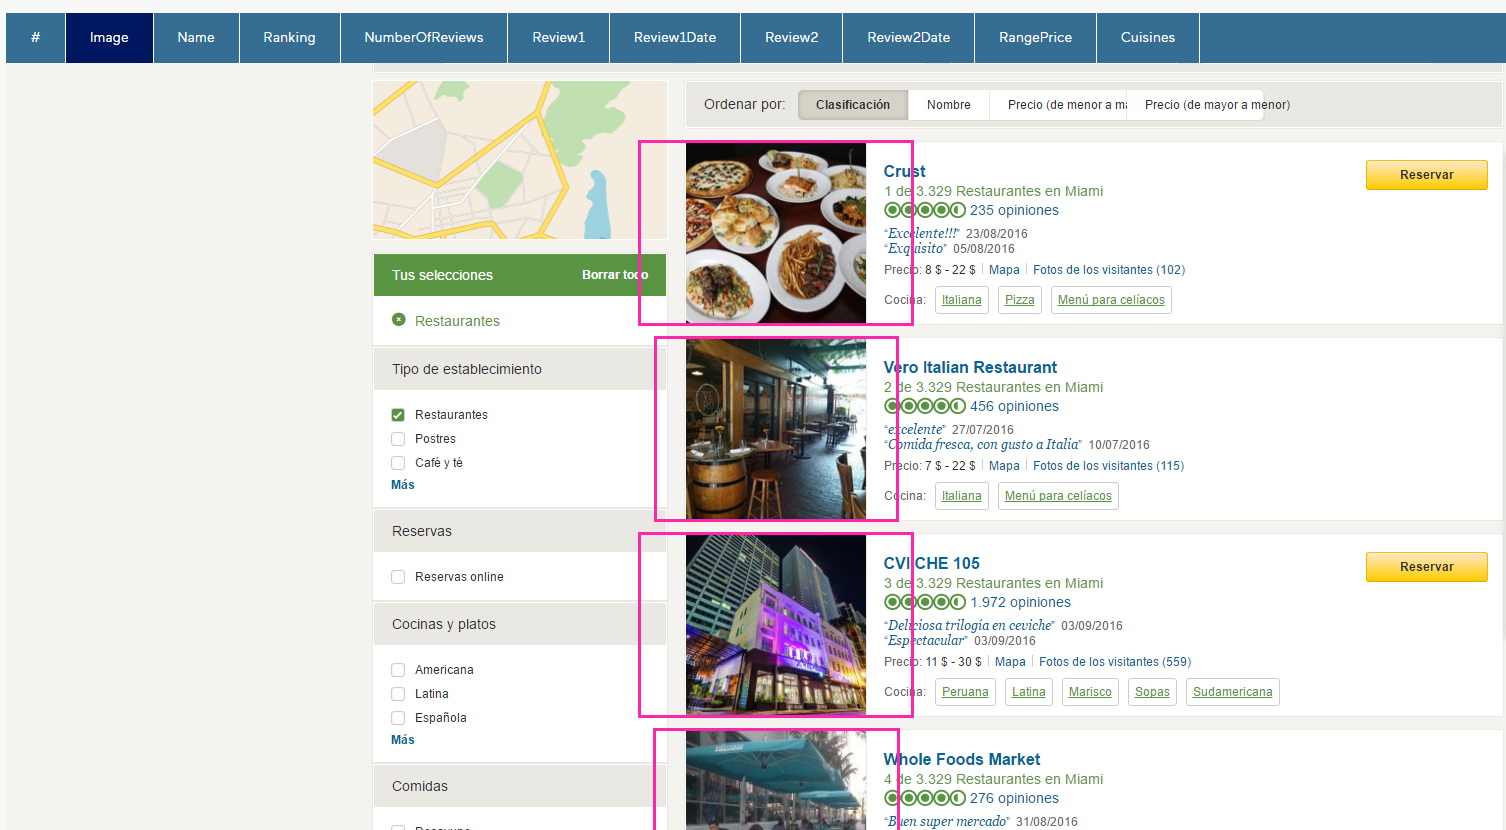
\includegraphics[width=0.8\textwidth]{./figs/ImportioEdit.png}
	\caption{Pantalla de edición de los elementos HTML a extraer en la tabla generada por import.io.}
	\label{fig:ImportioEdit}
\end{figure}

Como última característica, cabe destacar que import.io, en su versión de pago, permite la actualización automática de los cambios que se produjesen en la hoja de cálculo resultante. Es decir, en caso de que el sitio web cambiase, algo muy frecuente en sitios web de esta índole, import.io se encargaría de escanear y extraer la tabla con el formato que se haya preestablecido.

Al igual que existe import.io, existen otras herramientas para la extracción de datos en forma tabular:
\begin{itemize}
	\item \textbf{importhtml de Google Spreadsheets}\footnote{Extracción de datos con importhtml de Google SpreadSheets: \url{https://mashe.hawksey.info/2012/09/reshaping-importhtml-data-in-google-spreadsheet-using-query-and-transpose-formula/}}, menos potentes, pero mucho más sencilla de utilizar y con contenido actualizable.
	\item \textbf{Gneiss Spreadsheet} permite definir consultas y extraer datos en forma de tabla de un servicio web RESTful API \cite{Chang2014} con la funcionalidad de auto-actualización de los datos.
\end{itemize}

\chapter{Wit.ai: Procesamiento del lenguaje natural orientado a bots conversacionales}
\label{anx:witai}

Wit.ai se define como una herramienta de procesamiento del lenguaje, ya sea para texto como para voz. El objetivo de esta herramienta es funcionar de nexo entre el lenguaje que comprenden los humanos y las funcionalidades que dispone un sistema software, como lo puede ser un chatbot. Trabaja con diferentes lenguajes como el inglés o el castellano (en fase de desarrollo actualmente, aunque funciona relativamente bien). La principal virtud es que con poco trabajo Wit.ai empieza a funcionar como es esperado. Wit.ai funciona a base de entrenamiento, es decir, el desarrollador de la aplicación debe de ir introduciendo frases que el usuario utilizaría para hacer peticiones al sistema. A medida de que disponga de más frases más preciso será encontrando las intenciones (Intents) o entidades que los usuarios hayan introducido.

Respecto al trabajo referente a SheetChat, se ha delegado la tarea de desambiguación de Intents y reconocimiento de entidades a Wit.ai. Wit.ai permite tanto introducir frases de manera manual o esperar a recibir frases de los usuarios e ir corrigiendo desambiguaciones en las que se haya podido equivocar Wit.ai para mejorar su sistema de reconocimiento. En la Figura \ref{fig:WitaiInbox} se pueden observar dos mensajes introducidos por alguno de sus usuarios. El sistema ha reconocido tanto la entidad alumno como el Intent al que se refería el usuario. Sin embargo en la Figura \ref{fig:WitaiFallo} Wit.ai ha sido incapaz de obtener toda la información necesaria para resolver la pregunta del usuario. En la imagen superior ha reconocido erroneamente el Intent y no ha visto la entidad alumno (lo que indica que requiere más entrenamiento con frases de ese tipo). En la imagen inferior si ha sido capaz de reconocer adecuadamente el Intent, pero no ha podido obtener la entidad alumno, por lo que tendrá que preguntar por ella para dar respuesta al Intent.

\begin{figure}[htb]
	\centering
	\includegraphics[width=0.8\textwidth]{./figs/WitaiInbox.png}
	\caption{Wit.ai infiriendo de dos frases cuales son los Intents correspondientes para cada uno de ellos y cuál es la entidad Alumno.}
	\label{fig:WitaiInbox}
\end{figure}

\begin{figure}[htb]
	\centering
	\includegraphics[width=0.8\textwidth]{./figs/WitaiFallo.png}
	\caption{En la imagen de arriba Witai infiere erroneamente el Intent y no reconoce la entidad. En la inferior el usuario no ha proporcionado ninguna entidad, por lo que el chat tendrá que preguntar por ella.}
	\label{fig:WitaiFallo}
\end{figure}

Como se ha mencionado previamente, Wit.ai funciona en base a una confianza en las detecciones que ha hecho. En SheetChat se exige que el grado de confianza ha de ser mayor que 0.5 sobre 1 para que una inferencia se de por válida. En la Figura \ref{fig:WitaiConfianza} se puede observar como el grado de confianza de que \emph{María} es un alumno es de 0.99 y que el Intent es \emph{fisicaPonderadaPorEjercicio} únicamente de 0.71. Si se le ha entrenado adecuadamente, es muy probable que María sea un alumno y, con una confianza menor, que lo que se quiere es obtener la media ponderada de los ejercicios de física.

\begin{figure}[htb]
	\centering
	\includegraphics[width=0.8\textwidth]{./figs/WitaiConfianza.png}
	\caption{Respuesta del servicio de wit.ai cuando se le proporciona una frase. Remarcado en morado está el grado de confianza referente a la entidad alumno que ha detectado, de azul la del Intent.}
	\label{fig:WitaiConfianza}
\end{figure}




























% line in order to check if utf-8 is properly configured: áéíóúñ



\backmatter

\bibliography{gap-pfg}

\chapter{Agradecimientos}

En primer lugar, me gustaría agradecer a mi director de proyecto Óscar Díaz por confiar en mi para la realización de este TFM. Ha sabido guiarme correctamente a lo largo de la elaboración del trabajo, atendiendo a las consultas con un trato humano excepcional.

Asimismo, me gustaría agradecer a mis compañeros de trabajo dentro del grupo Onekin. Estos no solo me han brindado con su ayuda cuando la he necesitado, si no que también me han abierto las puertas de su grupo de par en par haciéndome sentir uno más del equipo.

De igual manera, quiero agradecer a mis compañeros de clase, de los que en poco tiempo he adquirido mucho conocimiento que me será útil para desarrollarme tanto profesionalmente como en el ámbito personal.

Por último, agradecer a mi familia, amigos, a Ainhoa y a mi entorno más cercano que una vez más han confiado en mi y me han respaldado en todo lo que he necesitado.

% In case we are using a glossary
% \glstoctrue
% \glsaddall
% \printglossaries

\end{document}
% line in order to check if utf-8 is properly configured: áéíóúñ
